\documentclass{article}

%%%%%%%%%%%%%%%%%%%%%%%%%%%%%%%%%%%%%%%%%%%%%%%%%%%%%%%%%%%%%%%%%%%%%%%%%%%%%%%%
%% package setup
%%%%%%%%%%%%%%%%%%%%%%%%%%%%%%%%%%%%%%%%%%%%%%%%%%%%%%%%%%%%%%%%%%%%%%%%%%%%%%%%



\usepackage{enumerate}
\usepackage[shortlabels]{enumitem}
\usepackage{amsfonts,amsmath, soul, matlab-prettifier, bm, amsthm,enumitem,amssymb,multirow,float,mathtools,bbm,array,varwidth,hyperref}
\usepackage[all]{xy}
\usepackage[margin=0.9in]{geometry}
\usepackage{graphicx}
\usepackage{mathtools}
\usepackage{tikz}
\usepackage{tikz-cd}
%\usepackage{bbold}
\usepackage[OT2,T1]{fontenc}
\usepackage{calrsfs}
\usepackage{dsfont}




\raggedbottom

%%%%%%%%%%%%%%%%%%%%%%%%%%%%%%%%%%%%%%%%%%%%%%%%%%%%%%%%%%%%%%%%%%%%%%%%%%%%%%%%
%% operators and symbols
%%%%%%%%%%%%%%%%%%%%%%%%%%%%%%%%%%%%%%%%%%%%%%%%%%%%%%%%%%%%%%%%%%%%%%%%%%%%%%%%

% operators
\newcommand{\Hom}{\mathrm{Hom}}
\newcommand{\Ker}{\mathrm{Ker}}
\newcommand{\Pic}{\mathrm{Pic}}
\newcommand{\Proj}{\mathrm{Proj}}
\newcommand{\rk}{\mathrm{rk}}
\newcommand{\Spec}{\mathrm{Spec}}
\newcommand{\Sym}{\mathrm{Sym}}
\newcommand{\Frob}{\mathrm{Frob}}
\newcommand{\Gal}{\mathrm{Gal}}
\newcommand{\GL}{\mathrm{GL}}
\newcommand{\SL}{\mathrm{SL}}
\newcommand{\Ind}{\mathrm{Ind}}
\newcommand{\Aut}{\mathrm{Aut}}
\newcommand{\Res}{\mathrm{Res}}
\newcommand{\Rep}{\mathrm{Rep}}
\newcommand{\Smo}{\mathrm{Smo}}
\newcommand{\Span}{\mathrm{Span}}
\newcommand{\supp}{\mathrm{supp}}
\newcommand{\trivial}{\mathbbm{1}}
\newcommand{\Irr}{\mathrm{Irr}}
\newcommand{\sign}{\mathrm{sign}}
\newcommand{\BSD}{\mathrm{BSD}}
\newcommand{\ord}{\mathrm{ord}}
\newcommand{\Reg}{\mathrm{Reg}}


% mathcal
\newcommand{\cO}{\mathcal{O}}

% mathbb
\newcommand{\CC}{\mathbb{C}}
\newcommand{\FF}{\mathbb{F}}
\newcommand{\NN}{\mathbb{N}}
\newcommand{\PP}{\mathbb{P}}
\newcommand{\QQ}{\mathbb{Q}}
\newcommand{\RR}{\mathbb{R}}
\newcommand{\ZZ}{\mathbb{Z}}
\newcommand{\GG}{\mathbb{G}}
\newcommand{\adele}{\mathbb{A}}
\newcommand{\pp}{\mathfrak{p}}

% mathfra
\newcommand{\fg}{\mathfrak{g}}
\newcommand{\fm}{\mathfrak{m}}


\newcommand{\norm}[1]{\left\lVert#1\right\rVert}
\newcommand{\hatv}[1]{\overset{\vee}{\mathstrut#1}}

% floor and ceiling
\DeclarePairedDelimiter\ceil{\lceil}{\rceil}
\DeclarePairedDelimiter\floor{\lfloor}{\rfloor}

\DeclareMathOperator{\Ima}{Im}


\linespread{1.5}

\theoremstyle{plain}
\newtheorem{thm}{Theorem}[section]
\newtheorem{question}[thm]{Question}
\newtheorem{prop}[thm]{Proposition}
\newtheorem{condition}[thm]{Condition}
\newtheorem{lemma}[thm]{Lemma}
\newtheorem{cor}[thm]{Corollary}
\newtheorem{algo}[thm]{Algorithm}
\theoremstyle{definition}
\newtheorem{defn}[thm]{Definition}
\newtheorem{notn}[thm]{Notation}
\newtheorem{rem}[thm]{Remark}
\newtheorem{example}[thm]{Example}
\newtheorem{examples}[thm]{Examples}
\newtheorem{fact}[thm]{Fact}

% some shortcuts
\RequirePackage{etoolbox}
%\AtEndEnvironment{remark}{\hfill$\lozenge$}
%\AtEndEnvironment{example}{\hfill$\lozenge$}

% Auxiliary commands
\DeclareMathSymbol{:}{\mathpunct}{operators}{"3A}%semicolon spaces
\RequirePackage{xspace}
\def\mat#1{\ensuremath{#1}\xspace}
\def\dmat#1#2{\gdef#1{\mat{#2}}}
\def\csdmat#1#2{\csdef{#1}{\mat{#2}}}

% Operators. Usage: \GL
\def\oper#1{\csdmat{#1}{\operatorname{#1}}}
\forcsvlist\oper{un, ord, tors, span, hol, rk, Ta, new, old,Jac, min,Rad, res, Tr,char, Det,Trace,GL,SL,deg,Hom,End,Vect,Mod,Rep,Ker,Im,Id,Gal,Aut, Frob,min, PGL, PSL, SO, sw, Ad}


% Mathbb Letters. Usage: \bA
\def\defbb#1{\csdmat{b#1}{\mathbb{#1}}}
\forcsvlist\defbb{1,A,B,C,D,E,F,G,H,I,J,K,L,M,N,O,P,Q,R,S,T,U,V,W,X,Y,Z}
\RequirePackage{bbm}
\dmat\bk{\mathbbm k}

% Mathcal Letters. Usage: \cA
\def\defcal#1{\csdmat{c#1}{\mathcal{#1}}}
\forcsvlist\defcal{A,B,C,D,E,F,G,H,I,J,K,L,M,N,O,P,Q,R,S,T,U,V,W,X,Y,Z,a,v}

% Mathfrak Letters. Usage: \fA
\def\defcal#1{\csdmat{f#1}{\mathfrak{#1}}}
\forcsvlist\defcal{A,B,C,D,E,F,G,H,I,J,K,L,M,N,O,P,Q,R,S,T,U,V,W,X,Y,Z,a,m,n,p,q, g, t}

% overline letters Usage \ovA
\def\defcal#1{\csdmat{ov#1}{\overline{#1}}}
\forcsvlist\defcal{A,B,C,D,E,F,G,H,I,J,K,L,M,N,O,P,Q,R,S,T,U,V,W,X,Y,Z,a,b,c,d,e,f,g,h,i,j,k,l,m,n,o,p,q,r,s,t,u,v,w,x,y,z}

% Greek letters
\dmat\al\alpha
\dmat\be\beta
\dmat\ga\gamma
\dmat\de\delta
\dmat\la\lambda
\dmat\ta\tau
\dmat\hi\chi
\dmat\eps\varepsilon
\dmat\vi\phi
\dmat\te\theta
\dmat\ksi\xi
\dmat\si\sigma
\dmat\om\omega
\dmat\Ga\Gamma
\dmat\La\Lambda

% Structures
\def\set#1{\left\{#1\right\}}
\def\sets#1#2{\left\{\left.#1\ \right\vert#2\right\}}
\def\rbr#1{\left(#1\right)}
\def\ang#1{\left\langle#1\right\rangle}
\def\n#1{\left\lvert#1\right\rvert}
\def\nn#1{\left\lVert#1\right\rVert}
\def\eq#1{\begin{equation}#1\end{equation}}
\def\ov#1#2{{\substack{#1\\#2}}} % #1 over #2

% Symbols
\def\mto{\mapsto}
\def\emb{\hookrightarrow}
\def\es{\emptyset}
\def\bs{\backslash}
\def\cupp{\smallsmile}
\def\surj{\twoheadrightarrow}

\newtheorem{conj}[thm]{Conjecture}
\newtheorem{notation}[thm]{Notation}

%Sha:
\usepackage[OT2,T1]{fontenc}
\DeclareSymbolFont{cyrletters}{OT2}{wncyr}{m}{n}
\DeclareMathSymbol{\Sha}{\mathalpha}{cyrletters}{"58}
%end of Sha

%\DeclareSymbolFont{cyrletters}{OT2}{wncyr}{m}{n}
%\DeclareMathSymbol{\Sha}{\mathalpha}{cyrletters}{"58}

%\DeclareMathAlphabet{\pazocal}{OMS}{zplm}{m}{n}


\title{Arithmetic Applications of Artin Twist and BSD}
\author{Edwina Aylward, Albert Lopez Bruch}

\begin{document}
	\maketitle
	\pagenumbering{arabic}
	\newpage
	\tableofcontents
	\newpage

\section*{Introduction}


\subsection*{Notation}
We use the following notation for characters:

\bigskip

\begin{tabular}{l | l}
    $R_{\bC}(G)$ & the ring of characters of representations of $G$ over $\bC$, \\
    $R_{\bQ}(G)$ & the ring of characters of representations of $G$ over $\bQ$, \\
    $\Irr_\bC(G)$ & the set of characters of complex irreducible representations of $G$, \\
    $\Irr_{\bQ}(G)$ & the set of characters of $\bQ$-irreducible representations of $G$, \\ 
    $\bQ(\rho)$ & the field of character values of a complex character $\rho$, \\
    $m(\rho)$ & the Schur Index of an irreducible complex character $\rho$ over $\bQ(\rho)$, \\
    \\
    $H^{x} = xHx^{-1}$ & for $H \leq G$ a subgroup of a group $G$ and $x \in G$,
\end{tabular}

\newpage
\section{Algebraic number theory and representation theory background}
\subsection{Representation theory of finite groups}\label{rep}

Let $G$ be a finite group. Recall that a \textbf{representation} of $G$ is a group homomorphism $\rho \colon G \to \GL(V)$ where $V$ is a complex vector space. Associated to a representation $\rho$ is a \textbf{character} $\chi \colon G \to \bC^{\times}$, defined by letting $\chi(g) = \Tr \rho(g)$ for $g \in G$. For complex represenations, $\rho$ is determined by its character; if $\rho$, $\rho'$ are representations with identical characters, then $\rho$ and $\rho'$ are isomorphic as representations. 

%Given a character $\chi$ of $G$, let $\bQ(\chi)$ be the smallest subfield of $\bC$ containing $\{ \chi(g) \mid g \in G \}$.
%Let $R_{\bC}(G)$ denote the ring of characters of complex representations of $G$. The number of complex irreducible representations of $G$ is equal to the number of conjugacy classes of $G$. Let $R_{\bQ}(G)$ be the ring of characters of rational valued representations of $G$.
%The number of irreducible $\bQ G$-representations up to isomorphism is equal to the number of conjugacy classes of cyclic subgroups of $G$. %(\cite[$\mathsection 13.1$, Cor. 1]{Serre})

Given an irreducible $\bQ G$-representation with character $\psi$, we have that 
\[\psi =  \sum_{\sigma \in \Gal(\bQ(\rho)/\bQ)}m(\rho)\cdot \rho^\sigma \]
for $\rho$ the character of an irreducible $\bC G$-representation, and $m(\rho)$ the Schur index.

In particular, the map $R_{\bC}(G) \to R_{\bQ}(G)$ given by sending an irreducible complex character $\rho$ to 
$\tilde{\rho} = \sum_{\sigma \in \Gal(\bQ(\rho)/\bQ)}m(\rho)\cdot \rho^\sigma$ is surjective.


Induction, Restriction\dots

\begin{thm}[Mackey Decomposition] 


\end{thm} 


\subsubsection{Permutation representations and the Burnside ring}

Let $G$ be a finite group. The \textbf{Burnside ring} $B(G)$ is the ring of formal sums of isomorphism classes of finite $G$-sets. We have addition by disjoint union: $[S] + [T] = [S \sqcup T]$, and multiplication by Cartesian product: $[S] \times [T] = [S \times T]$ for $S$, $T$ finite $G$-sets. 

There exists a bijection between the isomorphism classes of transitive $G$-sets and the conjugacy classes of subgroups $H \leq G$, where $H$ is the stabilizer of a point on which $G$ acts. Then any transitive $G$-set $X$ is isomorphic to the action of $G$ on $G/H$ for $H \leq G$, so that we can consider $B(G)$ to be a $\bZ$-module generated by the orbits of the action of $G$ on the elements $\{G/H : H \leq G\}$, where we consider $H$ up to conjugacy. For notational purposes, we then write elements $\Theta \in B(G)$ as $\Theta = \sum_i n_i H_i$ with $n_i \in \bZ$, $H_i \leq G$.

Given a transitive $G$-set $G/H$ for $H\leq G$, we can look at the permutation representation $\bC[G/H]$ . This defines a homomorphism from the Burnside ring to the rational representation ring $R_{\bQ}(G)$ of $G$: 
\[ \bC[-] \colon B(G) \to R_{\bQ}(G),  \ \ \ \ \ \sum_i n_i H_i \mapsto \bC[\sum_i n_i H_i ] = \sum_i n_i \Ind_{H_i}^G \trivial_{H_i}. \]

Elements in the kernel of this map are known as \textbf{Brauer relations}

{\color{red} define maps Ind, Res on the Burnside ring}
\subsection{Decompositions of primes in field extensions}
\subsection{Class field theory}
\subsubsection{Genus field}

In this section we introduce the concept of a genus field, as well as properites that will be useful for us.

Let $K$ be a number field. The \textbf{ideal class group} $\Cl_K = I_k / P_K$ is the group of fractional ideals quotiented by principal ideals.
For an ideal $\fp$, we let $[\fp]$ denote its class in $\Cl_K$.

The \textbf{extended ideal class group} is the group $\Cl_K^{+} = I_k / P_k^{+}$, where
$P_k^{+}$ denotes the subgroup of principal ideals with totally positive generator, i.e. ideals $\alpha \cO_k$ where $\sigma(\alpha) > 0$ for all real embeddings $\sigma \colon K \to \bR$.

Note that $\Cl_K^{+}$ is the ray class group for the modulus $\fm$ of $K$ consisting of the product of all real primes. The corresponding ray class field is known as the \textbf{extended Hilbert class field}, which we'll denote as $H^{+}$. Let $H$ be the usual Hilbert Class field of $K$. Then one has $H \subset H^{+}$. Moreover, the index can be described in terms of the structure of $K$:

\begin{thm}[Janusz 3. Extended Class group]
    Let $r$ be the number of real primes of $K$. Let $U_K$, $U_K^{+}$ the group of units and totally positive units of $K$ respectively, Then 
    \[ [H^{+} \colon H] = 2^r [U_K \colon U_K^{+}]^{-1} .\]
\end{thm}
For quadratic fields, the index depends on the norm of a fundamental unit:

\begin{cor}
    Let $K = \bQ(\sqrt{d})$ with $d$ a square-free positive integer. Let $\epsilon$ be a fundamental unit of $K$. Then $[H^{+} \colon H] = 1$ or $2$, according as $N_{K / \bQ}\left(\epsilon\right) = -1$ or $1$. 
\end{cor}
Observe that if $K$ has no real places, then $H^{+} = H$.

Fix $K = \bQ(\sqrt{d})$ for $d$ a squarefree integer. The (extended) Hilbert class field of $K$ need not be abelian over $\bQ$ (note that it is Galois by uniqueness of the (extended) Hilbert class field). However it can be convenient to consider the maximal subfield of $H$ that is Galois over $\bQ$. 

\begin{defn}
    For any abelian extension $K / \bQ$, the \textbf{genus field} of $K$ over $\bQ$ is the largest abelian extension $E$ of $\bQ$ contained in $H$. The \textbf{extended genus field } is the largest abelian extension $E^{+}$ of $\bQ $ contained in $H^{+}$.
\end{defn}

Let $\sigma \in \Gal(H^{+} / \bQ)$ be such that $\sigma|_{K}$ generates $\Gal(K / \bQ)$. $E$ has the following properties:

\begin{thm}[Janusz 3.3]\label{janusz-3.3}
    \begin{enumerate}
        \item $\Gal(H / E)$ is isomorphic to the subgroup of $C_K$ generated by the ideal classes of the form $[\sigma(\fU)\fU^{-1}]$, $\fU \in I_K$. 
        \item $\Gal(H / E) \simeq (C_K)^2$. 
    \end{enumerate}
\end{thm}

Note that this says that every class $[\sigma(\fU) \fU^{-1}]$ is a square in $C_K$.

This allows us to deduce the following:

\begin{thm} 
Let $p$ be a prime in $\bQ$. If the inertial degree of $p$ in $E / \bQ$ is $1$, then $p$ is the norm of a principal ideal in $K$. 
\end{thm} 

\begin{proof}
It's clear by inspection that $\Gal(E / K) = \Cl_K / \left(\Cl_K\right)^2$ is the maximal quotient of exponent $2$. Let $\fp$ be a prime of $K$ lying over $p$. Then $N_{K / \bQ}(\fp) = p$ and $\fp$ splits in $E$, so that $[\fp] \in (\Cl_K)^2$. Thus by theorem \ref{janusz-3.3} there is a fractional ideal $\fU$ of $I_K$ such that 
$[\fp] = [\sigma(\fU)\fU^{-1}]$. Observe that $N_{K / \bQ}(\sigma(\fU)\fU^{-1}) = 1$. It follows that $[\fp]^n$ is represented by a fractional ideal of norm $p$ for all $n$. Since $\Cl_K$ is finite, this implies there is a principal fractional ideal in $K$ of norm $p$. 
\end{proof}

The extended genus field $E^{+}$ is easier to describe than $E$.

\begin{thm} 
Suppose the discriminant of $K / \bQ$ has $t$ prime divisors. Then $C_K / (C_K)^2$ has order $2^{t-1}$ if $d < 0$ or if $d > 0$ and a unit of $K$ has norm $-1$. Otherwise, if $d>0$ and all units of $K$ have norm $1$, it has order $2^{t - 2}$.
\end{thm} 

\begin{thm} 
Let the discriminant of $K$ be $\Delta$ and suppose $|\Delta| = p_1 p_2 \cdots p_t$ where $p_2, \ldots p_t$ are odd primes, and $p_1$ is either odd or a power of $2$. Then the extended genus field of $K$ is 
    \[ E^{+} = \bQ(\sqrt{d}, p_2^*, \ldots p_t^*) = K(p_2^*, \ldots p_t^*), \] 
where 
\[ \begin{cases}
    p_i^* = \sqrt{p_i} & \mathrm{if }\ p_i \equiv 1 \pmod 4, \\
    p_i^* = \sqrt{-p_i} & \mathrm{if }\ p_i \equiv 3 \pmod 4
\end{cases}\]
\end{thm} 


\begin{cor}
    Let $q$ be a prime in $\bQ$, $K = \bQ(\sqrt{d})$ with discriminant $\Delta$ such that $|\Delta| = p_1 p_2 \cdots p_t$ as above. If $q \equiv 1 \pmod {|\Delta|}$, then $q$ is the norm of a principal ideal in $K$.
\end{cor}

\begin{proof}
    Any prime above $q$ in $K$ splits in $E^{+}$, hence also in $E$.
\end{proof}

We want to understand when $p$ is the norm of an element. Note that if $H = H^{+}$, then $p$ being the norm of an ideal guarantees that it is the norm of an element. If $-1$ is a norm in our field then we are also fine. 

\begin{thm}
    Let $K = \bQ(\sqrt{d}) \subset \bQ(\zeta_m)$ with $m$ odd. Suppose that $K$ is real. Then $-1$ is the norm of an element from $K$. 
\end{thm}

\begin{proof}{\color{red} be more specific}
    Any prime dividing $d$ is congruent to $1 \pmod 4$. 
    This implies that $d$ is the sum of two squares, which implies that $-1 = x^2 - d y^2$ for some $x, y \in \bQ$.
\end{proof}

Note that $-1$ being the norm of an element in $K$ does not ensure that $-1$ is the norm of a unit in $K$. The smallest counter-example is $K = \bQ(\sqrt{34})$. The element $\frac{5}{3} + \sqrt{34}$ has norm $-1$, but there is no unit with norm $-1$. 


\vspace{10em}

\begin{prop}
$\bQ(\sqrt{p^*})$ has odd narrow class number.
\end{prop}    

\begin{cor}\label{p-norm}
The prime $p \in \bQ$ is the norm of an element in $\bQ(\sqrt{p^*})^{\times}$.
\end{cor}

\newpage
\section{Proving things\dots}
\subsection{Norm relations}

Recall that in Section \ref{rep}, we associated to $\rho \in R_{\bC}(G)$ the character
    \[ \widetilde{\rho} = \sum_{\sigma \in \Gal(\bQ(\rho) / \bQ)} m(\rho) \rho^{\sigma} \quad \in R_{\bQ}(G) .\]
 Call $\Theta = \sum_i n_i H_i \in B(G)$ a \textbf{$\rho$-relation} if 
    \[ \sum_i n_i \Ind_{H_i}^G \trivial \simeq \widetilde{\rho}. \]
Given such a $\rho$, consider functions $\psi \colon B(G) \to \bQ^{\times} / N_{\bQ(\rho) / \bQ}(\bQ(\rho)^\times)$ (written multiplicatively). We say two functions $\psi$, $\psi'$ are \textbf{$\rho$-equivalent}, written $\psi \sim_{\rho} \psi'$, if $\psi / \psi'$ is trivial on all $\rho$-relations. 

If $\Theta \in \ker \psi$, then $\psi(\Theta)$ is the norm of an element from $\bQ(\rho)^{\times}$. We call an instance of this a \textbf{norm relation}.
In particular, when $\psi \sim_{\rho} 1$, then we obtain a norm relation for all $\rho$-relations $\Theta$. 

\begin{rem}
    If $\rho = 0$ then we call functions $\psi \sim_{\rho} 1$ \textbf{representation theoretic}. These have been studied in {\color{red} cite}.
\end{rem}

\begin{example}
  Take $\rho = 0$, and $V$ a representation of $G$. The function $\psi(H) = \dim V^H$ satisfies $\psi \sim_{\rho} 1$ as $\dim V^H = \langle \Res_{H} V , \trivial_H \rangle = \langle V, \Ind_{H}^G \trivial \rangle$ by Frobenius reciprocity.
\end{example}

\begin{example}
    Let $G = C_p$ for $p$ a prime. Let $\rho$ be a character of degree $p$. There is a unique $\rho$-relation given by $\Theta = C_1 - C_p$. Let $\psi(H) = [G \colon H]$. Then $\psi(\Theta) = p$, which is a norm from $\bQ(\zeta_p)$ by Corollary \ref{p-norm}. 
\end{example}

\begin{example}\label{cyclic-relns}
Let $G = C_n$. For each $d \mid n$, let $\chi_d = \widetilde{\varphi_d}$, where $\varphi_d$ is an irreducible complex character of $G$ with field of values $\bQ(\zeta_d)$ and kernel of index $d$.
Then $\{ \chi_d \colon d\mid n \}$ form a basis for the irreducible rational-valued representations of $G$. Note that $\Ind_{C_{n/ d}}^G \trivial$ is the direct sum of irreducible complex representations of $G$ contain $C_{n / d}$ in their kernel. Thus, $\Ind_{C_{n/ d}}^G \trivial \simeq \sum_{d' \mid d} \chi_{d'}$. Applying M\"{o}bius inversion, we obtain the unqiue $\varphi_d$-relation for each $d \mid n$:
\[ \chi_d = \sum_{d' \mid d} \mu(d / d') \cdot \Ind_{C_{n/ d}}^G \trivial. \]
\end{example}


\begin{example}
Let $E / \bQ$ be an elliptic curve, $G = \Gal(F / \bQ)$ for $F / \bQ$ a Galois extension. For $H \leq G$, the function $\psi \colon H \mapsto C(E / F^H)$ extends to a multiplicative function on the Burnside ring. Given a representation $\rho$ of $G$, one can ask when $\psi \sim_{\rho} 1$.
\end{example}

\subsubsection{D-local functions}\label{D-loc}

(This is taken from section 2.3 of Vlad and Tim's regulator constants paper.)

Consider $G = \Gal(F / \bQ)$ and intermediate field $F^H$ for $H < G$. Let $p$ be a prime with decomposition group $D$ in $G$. 
Then the primes above $p$ in $F^H$ correspond to double cosets $H\ G/ D$. If a prime $w$ in $F^H$ coresponds to the double coset $HxD$, then its decomposition and inertia groups in $F / F^H$ are $H \cap D^x$ and $H \cap I^x$ respectively. In partiular, the ramification degree and residue degree over $\bQ$ are given by $e_w = \frac{|I|}{|H \cap I^x|}$ and $f_w = \frac{[D \colon I]}{[H \cap D^x \colon H \cap I^x]}$. 

Our fudge factors $C(E / F)$ are defined locally; one has $C(E / F) = \prod_v c_v(E / F) \cdot |\omega / \omega_{v, \min}|$. Here $v$ runs over finite places of $F$, $\omega$ is a global minimal differential for $E / \bQ$, and $\omega_{v, \min}$ is a minimal differential at $v$.
Considering the function $H \mapsto C(E / F^H)$, and writing $C_p(E / F^H) =\prod_{v | p} c_v(E / F)\cdot |\omega / \omega_{v, \min}|$ one has

\[ \sum_{i} n_i H_i \mapsto \prod_i C(E / F^{H_i})^{n_i} = \prod_{p} C_p(E / F^H)^{n_i}. \]
Therefore, our function is the product of local functions for each $p$. Since $C_p(E / F^H)$ depends on $e_w$, $f_w$ for $w | p$, we are motivated to define the following:

\begin{defn}
    Suppose $I \triangleleft D < G$ with $D / I$ cyclic, and $\psi(e,f)$ is a function of $e, f \in \bN$. Define
    \[ \left(D, I, \psi\right) \colon \quad H \mapsto \prod_{x \in H\backslash G / D} \psi\left(\frac{|I|}{|H \cap I^x|}, \frac{[D \colon I]}{[H \cap D^x \colon H \cap I^x]}\right). \]
    Then, this is a function on the Burnside ring.
\end{defn}

\begin{example}
For semi-stable reduction, we're considering $\psi(e, f) = e$ (the Tamagawa number). For the $d_v$ terms in the case of additive potentially good reduction at p ($p$ not equal to $2$ or $3$), we consider $\psi(e, f) = p^{f \floor{e n /12}}$, where $n \in \{2,3,4,6,9,10\}$.
\end{example}




\subsection{Compatibility in odd order extensions}

Suppose that $G = \Gal(F / \bQ)$ has odd order, and $E / \bQ$ an elliptic curve with good reduction at wildly ramified primes in $F / \bQ$. We look at a relation of the form
\begin{equation}\label{reln} 
    \sum_i n_i \Ind_{H_i}^G \trivial \simeq \rho \oplus \tau(\rho),
\end{equation}
where $\rho$ is a character of $G$ with $\Gal(\bQ(\rho) / \bQ) = \langle \tau \rangle $ of size $2$. In particular we let $m$ denote the minimal positive integer such that $\bQ(\rho) \subset \bQ(\zeta_m)$. The sum on the left is over subgroups $H_i \subseteq G$. 

If I consider $\Res_D(\rho)$ where $D$ is a decomposition group of exponent $k$, then for $\Res_D(\rho)$ to be non-rationally valued, one needs $m \mid k$. Note that in the context of norm relations, if $\Res_D(\rho) = \Res_D(\tau(\rho))$, then we always get squares.

So now suppose that $D = I = C_n$ with $m \mid n$. Applying $\Res_D$ to (\ref{reln}), we get
\begin{equation}\label{reln-resD}
\sum_i n_i \sum_{x \in H_i \backslash G / D} \Ind_{D \cap x^{-1}H_i x}^D \trivial \simeq \Res_D \rho \oplus \tau(\Res_D \rho).
\end{equation}

Since both sides are now rationally valued, we can write this as $\sum_{d \mid n} a_d \cdot \chi_d$ where $a_d \in \bZ$ and $\{ \chi_d \colon d\mid n \}$ form a basis for the irreducible rational-valued representations of $D$. Explicitly, $\chi_d$ is the sum of the Galois conjugates of an irreducible complex character of $D$ with field of values $\bQ(\zeta_d)$ and kernel of index $d$ (which we'll write as $D_d$ ).

We can write each $\chi_d$ in terms of permutation modules:
\begin{equation}\label{chi-d} \chi_d = \sum_{d' \mid d} \mu(d' / d)\Ind_{D_d'}^D \trivial .\end{equation}
Substituting this into  $\sum_{d \mid n} a_d \cdot \chi_d$ gives an expression for the LHS of (\ref{reln}) (since cyclic groups have no Brauer relations, this is on the nose).
In particular, if we have a $D$-local function, we can evaluate it on each $\chi_d$-relation as in (\ref{chi-d}). Then the total expression is the product of these, raised to $a_d$.

Since we understand represntation theory of cyclic groups (wow!), we'd like to be able to reduce to cyclic decomposotion groups. Note that since we only assume bad reduction at tamely ramified primes in $F / \bQ$, one has that $I$ is cyclic. 
It turns out that we may assume that $D = I$ when $[D \colon I]$ is odd. 

\begin{lemma}\label{DeqI}
    In an odd degree unramified extension, Tamagawa numbers change only up to squares. In particular, if $[D \colon I]$ is odd, then $(D, I, \psi) \sim_{\rho} (I, I, \psi)$ for any $\rho$ with $\bQ(\rho)$ even, where $\psi(e,f)$ is the Tamagawa number. 
\end{lemma}

\begin{proof}
    Yadada
\end{proof}

\subsubsection{Semistable reduction}

In this subsection we work towards proving the following:

\begin{thm}
    Let $F / \bQ$ be a Galois extension of odd degree, with $G = \Gal(F / \bQ)$. 
    Consider a semistable elliptic curve $E / \bQ$ with good reduction at primes that are wildly ramified in $F / \bQ$.
    
    Then, for any $\rho \in R_{\bC}(G)$ with $[\bQ(\rho)\colon \bQ] > 1$, the function $f \colon B(G) \to
    \bQ^{\times} / N_{\bQ(\rho) / \bQ}(\bQ(\rho)^{\times})$ sending $H \mapsto C(E / F^{H})$ satisfies $f \sim_{\rho} 1$.
\end{thm}

\subsubsection{dv terms in additive reduction}


\subsubsection{Tamagawa numbers in additive reduction}

We use the following description of Tamagawa numbers. %Tim and Vlad reg consts Lemma 3.19

\begin{lemma}
    Let $K' /K / \bQ_p$ be finite extensions and $p \geq 5$. Let $E / K$ be an elliptic curve with addtive reduction; 
    \[ E \colon y^2 = x^3 + Ax + B, \]
    with discriminant $\Delta = -16(4 A^3 + 27 B^2)$. Let $\delta = v_K(\Delta)$, and $e = e_{K' / K}$.

    If $E$ has potentially good reduction, then 
        \[
        \begin{array}{l l l l}
            \gcd(\delta e, 12) = 2 & \implies & c_v(E / K') = 1, & \quad (II, II^*) \\
            \gcd(\delta e, 12) = 3 & \implies & c_v(E / K') = 2, & \quad (III, III^*) \\
            \gcd(\delta e, 12) = 4 & \implies & c_v(E / K') = \begin{cases} 1, & \sqrt{B} \notin K'
                                \\ 3, & \sqrt{B} \in K' \end{cases}, & \quad (IV, IV^*) \\
            \gcd(\delta e, 12) = 6 & \implies & c_v(E / K') = \begin{cases} 2, & \sqrt{\Delta} \notin K'
                \\ 1 \ \text{or} \ 4, & \sqrt{\Delta} \in K' \end{cases}, & \quad (I_0^*) \\
            \gcd(\delta e, 12) = 12 & \implies & c_v(E / K') = 1. & \quad (I_0)
        \end{array}
        \]
    Moreover, the extensions $K'(\sqrt{B}) / K'$ and $K'(\sqrt{\Delta}) / K'$ are unramified.
\end{lemma}

So suppose an elliptic curve $E / \bQ$ has additive reduction at $p$, with $p \geq 5$. Then we can write $E \colon y^2 = x^3 + Ax + B$. Let $D = \Gal(F_{\fp} / \bQ_p)$ be the local Galois group at $p$. Assume that $p$ is totally tamely ramified, so that $D = I = C_n$. Since there is no wild ramification, and $f = 1$, this means that $n \mid p - 1$. We consider the contribution corresponding to an irreducible rational character $\chi_d$ of $D$, given by 
\begin{equation}\label{tam-contrib}
\prod_{d ' \mid d} C(E / F_{\fp}^{D_{d'}})^{\mu(d / d')}.
\end{equation}

Observe that in a totally ramified extension of degree coprime to $12$, the Tamagawa number remains the same. If $(12, d) = 1$, then $(12, d') = 1$ for $d' \mid  d$, so the Tamagawa number is consant accross subfields $F_{\fp}^{D_{d'}}$. Therefore,
\[\prod_{d ' \mid d} C(E / F_{\fp}^{D_{d'}})^{\mu(d / d')} = C(E / \bQ_p)^{\sum_{d' \mid d} \mu(d / d')} = 1,\]
assuming $d > 1$. 

So we only need to worry about when $3 \mid d$. If we have type $III$ or $III^*$ or $I_0^*$ then the Tamagawa number is still unchanged in any totally ramified cyclic extension of degree dividing $d$. We will treat the other cases seperately: 

\vspace{1em}

\noindent\underline{\textit{Type $II$ and $II^*$ reduction:}}

Firstly, suppose that $\delta = 2$, that is we have Type $II$ reduction. If $3 \mid d'$ then $E / F_{\fp}^{D_{d'}}$ has type $I_0^*$ reduction. The Tamagawa number then depends on whether $\sqrt{\Delta} \in \bQ_p$. Since we have additive reduction, we know that $p \mid A$, $p \mid B$. Moreover, $\delta = 2$ implies that $v_p(B) = 1$. Then, $\Delta = p^2\cdot \alpha$, and $\alpha \equiv -27\cdot\square \pmod p$. Therefore $\sqrt{\Delta} \in \bQ_p \iff -3$ is a square $\pmod p$. But this is the case; we assumed $p \equiv 1 \pmod n$, so $p \equiv 1 \pmod 3$. Therefore the Tamagawa number will be $1$ or $4$, which is a square.
If $3 \nmid d'$ then the reduction type over $ F_{\fp}^{D_{d'}}$ is $II$ or $II^*$. Then the Tamagawa number is $1$. Thus in total, we get a square contribution from (\ref{tam-contrib}).

If $\delta = 10$, then $E / F_{\fp}^{D_{d'}}$ has reduction type $I_0^*$ whenever $3 \mid d'$. Once more, $v_p(A), v_p(B) \geq 1$, and $v_p(\Delta) = 10 = \min(3 v_p(A), 2 v_p(B))$ {\color{red} maybe this is suss} $\implies v_p(B) = 5$. Therefore we get $\Delta = p^{10} \alpha$ with $\alpha \equiv -27\cdot\square \pmod p$, and we conclude as above.

\vspace{1em}

\noindent\underline{\textit{Type $IV$ and $IV^*$ reduction:}}

Now, if $E /\bQ_p$ has additive reduction of type $IV$ or $IV^*$, it attains good reduction over any totally ramified cyclic extension of degree divisible by $3$. This could result with $3$ coming up an odd number of times in our Tamagawa number product, when $\sqrt{B} \not\in \bQ_p$. 

%We show that for both types, one has $\sqrt{B} \in \bQ_p$. 
%Indeed, if $\delta = 4$, then $v_p(B) = 2$, and $v_p(A) \geq 2$. 
\vspace{1em}
In summary, 
\begin{equation}
    \prod_{d ' \mid d} C(E / F_{\fp}^{D_{d'}})^{\mu(d / d')}
    = 
    \begin{cases}
        1 & 3 \nmid d, \\
        1 & 3 \mid d, \delta \in \{0, 3, 6, 9\}, \\
        1 \cdot \square & 3 \mid d, \delta \in \{2, 10\}, \\
        3^a \cdot\square, a \in \{0,1\} & 3 \mid d, \delta \in \{4,8\}.
    \end{cases}
\end{equation}

(There's no reason why we can't get 3; see elliptic curve 441b1 with additive reduction at $7$ of type IV and Tamagawa number equal to $3$)

However, it turns out we will only get $3$ occuring oddly when $d = 3$. Indeed, one has that $\langle \Ind_{D_{d'}}^D \trivial, \psi_3 \rangle = 1$ if $3 \mid d'$, and $0$ if $3 \nmid d'$, where $\psi_3$ is an irreducible character of $D$ of order $3$. Therefore one sees that the number of places with ramification degree divisible by $3$ cancels unless $d = 3$. Indeed, $\langle \chi_d , \psi_3 \rangle = 0$ unless $d = 3$, 
in which case it is $1$. Therefore (\ref{tam-contrib}) can only be non-square when $d = 3$.


\newpage
\section{Representations, L-functions and Artin Twists}
\subsection{Artin Representations and  \texorpdfstring{$\ell$}{TEXT}-adic Representations} \label{subsection_reps}

The Birch-Swinnerton-Dyer conjecture classically provides a connection between the arithmetic of elliptic curves and their $L$-functions. In this prelimiary section, we explore the classical definition of $L$-functions attached to an elliptic curve and their twists, and we explore some of the relevant properties that we will use later on. To do so, we first need to explore the notion of an Artin representation and of an $\ell$-adic representation. 

Throughout this section we fix a field $K$, which will either be a number field or a local field of characteristic $0$. We also fix an algebraic closure $\hat{K}$ of $K$ and we denote by $G_K$ the absolute galois group $\Gal(\bar{K}/K)$ of $K$. We recall that $G_K$ is a profinite group
$$G_K=\varprojlim_{F}\Gal(F/K),$$
where $F$ ranges over the finite Galois extensions of $K$ and therefore has a natural topology where a basis of open sets is given by $\Gal(\bar{K}/F)$ where $F$ is a finite extension of $K$.

\begin{defn}
    Let $K$ be a number field or a local field with characteristic $0$. An \textbf{Artin representation} $\rho$ over $K$ is a complex finite-dimensional vector space $V$ together with a homomorphism $\rho:G_K\to\GL(V)=\GL_n(\CC)$ such that there is some finite Galois extension $F/K$ with $\Gal(\bar{K}/F)\subseteq\ker\rho$. In other words, $\rho$ factors through $\Gal(F/K)$ for some finite extension $F$ of $K$.
\end{defn}

Hence, an Artin representation can be equivalently viewed as a finite dimensional representation of $\Gal(F/K)$ where $F$ is some finite Galois extension of $K$. Throughout the document, we will use both notions depending of the context, and refer to either of them as Artin representations.

\begin{rem}
    The condition above that $\Gal(\bar{K}/F)\subseteq\ker\rho$ is equivalent to $\ker\rho$ being open in $G_K$. This clearly implies that $\rho$ is a continuous homomorphism of topological groups. Surprisingly, the converse is also true: a continous homomorphism $\rho:G_K\to\GL_n(\CC)$ has open kernel. The proof of this result relies on the fact that `small' neighbourhoods of the identity in $\GL(V)=\GL_n(\CC)$ do not contain any non-trivial subgroups. Hence, if $\phi:G_K\to\GL(V)$ is continous and $U$ is such a neighbourhood in $\GL(V)$, then $\phi^{-1}(U)\subseteq\ker\phi$ and $\phi^{-1}(U)$ is open, showing that $\ker\rho$ is open too. Hence the above condition is equivalent to continuity of $\rho$ with respect to the natural topologies.
\end{rem}

Next, we define the notion of an $\ell$-adic representation, which will be needed to define the $L$-function of an elliptic curve.

\begin{defn}
    Let $K$ be a number field or a local field of characteristic $0$. A \textbf{continuous $\ell$-adic representation} $\rho$ over $K$ is a continous homomorphism $\rho:G_K\to\GL_n(F)$ where $F$ is a finite extension of $\QQ_\ell$.
\end{defn}

\begin{rem} \label{rem_cont_ladic}
    The topologies on $\GL_n(\CC)$ and $\GL_n(\QQ_\ell)$ are very different, and in particular and $\ell$-adic representation may not have an open kernel. Instead, continouity is equivalent to the following condition: for every $m\geq1$, there is some finite field extension $F_m$ of $K$ such that for all $g\in\Gal(\bar{K}/F_m)$, $\rho(g)\equiv \mathrm{Id}_n\pmod{\ell^m}$.
\end{rem}

Given an Artin representation $\rho$, one can view it as homomorphism $\rho:G_K\to\GL_n(\bar{\QQ})$ and since it factors through a finite quotient, we can realise it as $\rho:G_K\to\GL_n(F)$ for some number field $F$. Hence, if $\ell$ is any rational prime and $\mathfrak{l}$ is a prime in $F$ above $\ell$, then one can realise $\rho$ as an $\ell$-adic representation $$\rho:G_K\longrightarrow\GL_n(F_\mathfrak{l}),$$
which is continous since $\rho$ factors through a finite quotient. Furthermore, Artin and $\ell$-adic representations over $K$ have more structure; namely, one can take \textbf{direct sums} and \textbf{tensor products}.

We describe the construction for Artin representations, since the $\ell$-adic case is completely analogous. Suppose we have two Artin representations $\rho_1,\rho_2$ over $K$, and by the discussion on the preceeding paragraph we can realise them as maps $\rho_i:G_K\to\GL_{n_i}(L_i),\ i=1,2$ where $L_1$ and $L_2$ are number fields. If we let $L=L_1L_2$, then the natural maps $\rho_1\oplus\rho_2:G_K\to\GL_{n_1+n_2}(L)$ and $\rho_1\otimes\rho_2:G_K\to\GL_{n_1n_2}(L)$ are both Artin representations. One can also show that this construction is also well-defined up to equivalence.

\subsection{Local Polynomials and L-functions}
We now briefly discuss how to attach analytic objects to Artin and $\ell$-adic reperesentations. These objects are usually described locally first, and then this local information is put together to get a global object. 

To begin, let $K$ be a local field with $0$ characteristic and let $p$ be the characteristic of the residue field $\kappa$. Let $\rho:G_K\to\GL(V)$ be an Artin or $\ell$-adic representation such that $\ell\neq p$ (this is an important technical assumption that we will not discuss further). By the \textbf{section on algebraic number theory} we have a short exact sequence
$$0\longrightarrow I_K\longrightarrow \Gal(\bar{K}/K)\xlongrightarrow{\epsilon} \Gal(\bar{\kappa}/\kappa)\cong\tilde{\ZZ}\longrightarrow 0,$$
where under the last isomorphism $1\in\tilde{\ZZ}$ corresponds to the map $\phi:\bar{\kappa}\to\bar{\kappa}$ where $x\mapsto x^p$ and this map is a topological generator of $\Gal(\bar\kappa/\kappa)$. Any preimage of $\phi$ under $\epsilon$ is called a Frobenius element $\Frob_K$ and it is therefore well-defined up to $I_K$. Furthermore, the space of intertia-invariants 
$$V^{I_K}:=\{v\in V:\rho(g)v=v\text{ for all }g\in I_K\}$$
is naturally a $G_K/I_K$ representation, which we denote $\rho^{I_K}$. we are now ready to define the local polynomial attached to $\rho$.

\begin{defn}
    Let $K$ be a local field of characteristic $0$ and let $p$ the characteristic of its local field. If $\rho$ is an Artin or $\ell$-adic representation such that $\ell\neq p$. Then the local polynomial attached to $\rho$ is
    $$P(\rho,T):=\det\left(I-T\cdot\rho^{I_K}\left(\Frob_K^{-1}\right)\right).$$  
\end{defn}

If $K$ is instead a number field, the idea is to consider all finite places of $K$ and consider all the local polynomials attached to all local completions of $K$ to build the corresponding L-function. More concretely, let $\rho:G_K\to\GL(V)$ be an Artin or $\ell$-adic representation and let $\pp$ be a finite place of $K$ and $K_\pp$ be the corresponding completion. Since $G_{K_\pp}=\Gal(\bar{K_\pp}/K_\pp)$ is naturally a subgroup of $G_K$, we can restrict $\rho$ to $\Res_\pp\rho:G_{K_\pp}\to\GL(V)$ and then calculate the corresponding local polynomial as long as $\pp$ and $\ell$ are coprime. If $\rho$ is an Artin representation, this allows us to construct the associalted $L$-function.

\begin{defn}
    Let $K$ be a number field and $\rho$ an Artin representation over $K$. If $\pp$ is a finite place of $K$, we denote the local polynomial at $\pp$ as 
    $$P_\pp(\rho,T):=P(\Res_\pp\rho,T).$$
    The associated $L$-function to $\rho$ is 
    $$L(\rho,s):=\prod_{\pp\text{ prime}}\frac{1}{P_\pp(\rho,N(\pp)^{-s})}.$$
\end{defn}

However, if $\rho$ is an $ell$-adic representation, constructing a global object is harder, since the above method does not yield information at the finite places $\pp$ that divide $\ell$. This motivates the following important definition.

\begin{defn}
    Let $\{\rho_\ell\}_{\ell\text{ prime}}$ be a family of $\ell$-adic representations for each prime $\ell$. We then say that $\{\rho_\ell\}_\ell$ is a \textbf{weakly compatible system of $\ell$-adic representations} if for every finite place $\pp$ of $K$ and rational primes $\ell,\ell'$ not divisible $\pp$, 
    $$P_\pp(\rho_\ell,T)=P_\pp(\rho_{\ell'},T)$$.
\end{defn}

When $\{\rho_\ell\}_\ell$ is a weakly compatible system of $\ell$-adic representations, the local polynomial $P_\pp(\rho_\ell,T)$ can be computed using any $\ell$ not divisible by $\pp$. This also allows us to define the $L$-function in this context.

\begin{defn}
    Let $K$ be a number field and let $\{\rho_\ell\}_\ell$ be a weakly compatible system of $\ell$-adic representations. Then the $L$-function attached to the system is 
    $$L(\{\rho_\ell\}_\ell, s)=\prod_{\pp\text{ prime}}\frac{1}{P_\pp(\{\rho_\ell\},N(\pp)^{-s})}.$$
\end{defn}




\subsection{The Tate Module of an Elliptic Curve and their L-function}
Let $K$ be a number field or a local field with characteristic $0$ \textbf{(Maybe for this section we should only assume K is a number field? Otherwise I don't know if it makes sense to talk about their L-function)} and fix an algebraic closure $\bar{K}$ of $K$. Let $E$ be an elliptic curve defined over $K$. To avoid notational confusion, whenever we write $E$ we refer to all of its $\bar{K}$ points, while $E(K)$ refers only to the $K$-rational points. The aim of this section is to describe a procedure to attach an $L$-function to a given elliptic curve over $K$. In order to achieve this, we will first construct a $2$-dimensional $\ell$-adic representation attached to $E$, and then construct the $L$-function as described in the section above.
Let $\ell$ be a rational prime number. For any $n\geq1$, we denote by $E[\ell^n]$ to be the $\ell^n$-torsion points; in other words, $E[\ell^n]$ is the kernel of the map $E[\ell^n]:E\to E$. We then have the diagram of compatible maps
\[
    \longrightarrow E[\ell^{n+1}]\xlongrightarrow{[\ell]} E[\ell^{n}]\xlongrightarrow{[\ell]}\cdots\xlongrightarrow{[\ell]} E[\ell^2]\xlongrightarrow{[\ell]} E[\ell]\xlongrightarrow{[\ell]} \{\mathcal{O}_E\} 
\] 
and therefore we can construct the inverse limit of this diagram
$$T_\ell(E):=\varprojlim_{n}E[\ell^n],$$
denoted as the $\ell$-adic Tate module of the elliptic curve $E$. By the uniformization theorem, we know that 
$$E[\ell^n]\cong\frac{\ZZ}{\ell^n\ZZ}\oplus\frac{\ZZ}{\ell^n\ZZ}$$
as groups, and therefore 
$$T_\ell(E)\cong\ZZ_\ell\oplus\ZZ_\ell$$
as $\ZZ_\ell$-modules. In addition, the Tate module carries important extra structure, namely the action of the absolute Galois group $G_K$. Since $E$ is defined over $K$, and the multiplication by $m$ maps are determined by polynomials with coefficients in $K$, there is a well-defined additive action $\psi_n:G_K\rightarrow\Aut_{\ZZ}(E[\ell^n])$. Furthermore, one can show that this actions are compatible with the inverse limit diagram of the Tate module. That is, for every $n\geq 1$ and $\sigma\in G_K$, the diagram


\begin{center}
    \begin{tikzcd}
        E[\ell^{n+1}] \arrow[d, "\psi_{n+1}(\sigma)"] \arrow[r, "\ell"] & E[\ell^n] \arrow[d, "\psi_n(\sigma)"]\\
        E[\ell^{n+1}] \arrow[r, "\ell"] & E[\ell^n]
    \end{tikzcd}
\end{center}

commutes. Therefoere, the actions $\psi_n$ induce an action of $G_K$ on $T_\ell(E)$ and since $T_\ell(E)\cong\ZZ_\ell\oplus\ZZ_\ell$, this corresponds to a $2$-dimensional $\ell$-adic representations
$$\psi_{E,\ell}:G_K\longrightarrow \GL_2(\ZZ_\ell)\subseteq\GL_2(\QQ_\ell).$$
We will also denote from now on $\rho_{E,\ell}$ to be the dual representation of $\psi_{E,\ell}$. For technical reasons we will not discuss, the $L$-function is tipycally constructed using the later ones.

\begin{rem}
    The representation above does indeed satisfy the conditions in Remark \ref{rem_cont_ladic}. In particular, given any $n\geq 1$, the field $F_n:=K(E[\ell^n])$ is a finite extension of $K$ since it is obtained by attaching finitely many algebraic numbers. By construction, $\Gal(\bar{K}/F_n)$ acts trivially on $E[\ell^n]$ and thus $\rho_{E,\ell}(g)\equiv \mathrm{Id}\pmod{\ell^n}$ for all $g\in\Gal(\bar{K}/F_n)$.
\end{rem}

Of course, the above construction can be followed by any rational prime $\ell$, and this gives a family $\{\rho_{E,\ell}\}_\ell$. To build an $L$-function as described in the section above, we would need this family to be weakly compatible. Thankfully, this and much more is true, and the next theorem collects the relevant results.

\begin{thm}
    Let $E$ be an elliptic curve over a number field $K$ and $\rho_{E,\ell}$ be the dual representation on $T_\ell(E)$. For every finite place $\pp$ of $K$, let $\kappa_\pp$ be the residue field of $K_\pp$, $q_\pp=|\kappa_\pp|$ and $a_\pp=1+q_\pp-|\tilde{E}(\kappa_\pp)|$. Then for any $\pp$ not diving $\ell$,
    \begin{align*}
        P_\pp(\rho_{E,\ell},T) & = 1-a_\pp T+q_p T^2, & \text{if } E/K_\pp \text{ has good reduction,}\\
        & = 1-T, & \text{if } E/K_\pp \text{ has split multiplicative reduction,}\\
        & = 1+T, & \text{if } E/K_\pp \text{ has non-split multiplicative reduction,}\\
        & = 1, & \text{if } E/K_\pp \text{ has additive reduction.}
    \end{align*}

    In particular, for any $\ell,\ell'$ not divisible by $\pp$, 
    $$P_\pp(\rho_{E,\ell},T)=P_\pp(\rho_{E,\ell'},T),$$
    and so $\{\rho_{E,\ell}\}$ is a weakly compatible system of $\ell$-adic representations.
\end{thm}

This allows us to define the $L$-function of an elliptic curve as above.

\begin{defn}
    Let $E$ be an elliptic curve over $K$. Then the $L$-function attached to $E$ is 
    $$L(E/K,s)=L(\{\rho_{E,\ell}\},s)=\prod_{\pp\text{ prime}}\frac{1}{P_\pp(\rho_{E,\ell},N(p)^{-s})}$$
\end{defn}

\subsection{Artin Twists of L-functions of Elliptic Curves}

We have already seen that given an elliptic curve over a number field $K$, one can construct the $L$-function $L(E/K,s)$. However, given an Artin representation $\rho$ over $K$, it is possible to attach more analytic objects, with remarkable arithmetic properties. We outline the main results below, without proofs. \textbf{Insert here relevant reference}. 

Fix some number field $K$, an elliptic curve $E$ over $K$ and an Artin repesentation $\rho$. Then, similary to the previous section, it is possible to show that $\{\rho_{E,\ell}\otimes\rho\}_\ell$ is also a weakly compatible system of $\ell$-adic representations. The corresponding $L$-function
$$L(E,\rho,s)=L(\{\rho_{E,\ell}\otimes\rho\},s)$$
is denoted as the \textbf{Artin-twist} of $L(E,s)$ by $\rho$. These objects have remarkable (both proven and conjectural) properties that we describe now.

\begin{thm}[Artin Formalism]
    Let $E$ be an elliptic curve over a number field $K$.
    \begin{enumerate}
        \item For Artin representations $\rho_1,\rho_2$ over $K$,
        $$L(\rho_1\oplus\rho_2,s)=L(\rho_1,s)L(\rho_2,s)\quad and\quad L(E/K,\rho_1\oplus\rho_2,s)=L(E/K,\rho_1,s)L(E/K,\rho_2,s)$$
        \item If $L/K$ is a finite extension and $\rho$ is an Artin representation over $L$, then $\Ind_{G_L}^{G_K}\rho$ is an Artin representation over $K$ and 
        $$L(\rho,s)=L(\Ind_{G_L}^{G_K}\rho,s)\quad and\quad L(E/L,\rho,s)=L(E/L,\Ind_{G_L}^{G_K}\rho,s).$$
        \item If $L/K$ is a finite extension as above and 
        $$\Ind_{G_L}^{G_K}\mathds{1}\cong\bigoplus_i\rho_i,$$
        then
        $$L(E/L,s)=\prod_i L(E/K,\rho_i,s).$$
    \end{enumerate}
\end{thm}

To simply notation, given any Artin representation $\rho$ over $L$ we will write $\Ind_{L/K}\rho$ instead of $\Ind_{G_L}^{G_K}\rho$. Furthermore if $F$ is a finite Galois extension of $K$ such that $\rho$ factors through $\Gal(F/L)$, then $\Ind_{L/K}\rho$ factors through $\Gal(F/K)$ and 
$$\Ind_{L/K}\rho\cong\Ind_{\Gal(F/L)}^{\Gal(F/K)}\rho.$$

Furthermore, as mentioned after Remark \ref{rem_cont_ladic}, by fixing some basis $\mathcal{B}$ of $V$ any Artin representation $\rho$ can be viewed as a representation $\rho:G_K\to\GL_n(F)$ for some number field $F$. The smallest such field is the \textbf{field of values} of $\rho$ and denoted by $\QQ(\rho)$. Any $\sigma\in\Gal(\QQ(\rho)/\QQ)$ induces a homomorphism $\sigma:\GL_n(\QQ(\rho))\to\GL_n(\QQ(\rho))$ and also a map
\begin{align*}
    \rho^\sigma:G_K &\longrightarrow\GL_n(F)\\
    g&\longmapsto \sigma(\rho(g)),
\end{align*}
which is another Artin representation, denoted as the twist of $\rho$ by $\sigma$.

\begin{conj}[Galois Equivariance of L-Twists]
    I need to check the precise statement of this result. This may need to come after the discussion on BSD.
\end{conj}


\section{Birch and Swinnerton-Dyer and Other Conjectures}
The Birch--Swinnerton-Dyer conjecture classically provides a connection between the arithmetic of elliptic curves and their $L$-functions. We have already investigated the construction and main results of the `$L$-functions side', and now we turn out attention to statement of the conjecture and towards understanding the arithmetic terms present in the conjecture. Some arithmetic terms present in the conjecture are easier to describe if the elliptic curve has a global minimal Weierstrass equation. Since we will be mainly interested in elliptic curves over $\QQ$, and in view of Proposition \ref{prop_globmin}, we will assume throughout that $E$ is an elliptic curve over $\QQ$ with \textbf{global minimal Weierstrass equation}
$$E:y^2+a_1xy+a_3y=x^3+a_2x^2+a_4x+a_6$$ 
for some $a_1,a_2,a_3,a_4,a_6\in\ZZ$, and let 
$\omega= dx / (2y+a_1x+a_3)$
be the associated \textbf{global minimal differential}.

\subsection{BSD and the Arithmetic Terms}

The Birch-Swinnerton-Dyer conjecture states the following.

\begin{conj}[BSD]
    Let $E$ be an elliptic curve defined over a number field $K$. Then 
    \begin{enumerate}[label={\bfseries  BSD\arabic*.}]
        \item The rank of the Mordell-Weil group of $E$ over $K$ equals the order of vanishing of the $L$-function; that is,
        $$\ord_{s=1}L(E/K,s)=\rk E/K.$$
        \item The leading term of the Taylor series at $s=1$ of the $L$-function is given by 
        \begin{equation}\label{BSD_2}
            \lim_{s\to1}\frac{L(E/K,s)}{(s-1)^r}\cdot\frac{\sqrt{|\Delta_K|}}{\Omega_+(E)^{r_1+r_2}|\Omega_-(E)|^{r_2}}=\frac{\Reg_{E/K}|\Sha_{E/K}|C_{E/K}}{|E(K)_{\tors}|^2}.
        \end{equation}
    \end{enumerate}
\end{conj}

We briefly explore the arithmetic invariants that appear as part of the statement of BSD2. Some of these invariants depend only on the number field $K$. These are the discriminant $\Delta_K$ of $K$ and the numbers $r_1$ and $r_2$, corresponding to the number of real and complex embeddings of $K$. A basic formula states that if $n=[K:\QQ]$, then $r_1+2r_2=n$. 

The other factors are arithmetic values related to the elliptic curve $E$. Importantly, here we assume that $E$ has rational coefficients.

\begin{enumerate}
    \item \textbf{Periods: } For elliptic curves $E$ defined over $\QQ$, there is a conjugation map $E\to E$, $P\mapsto\bar{P}$. We then define $E(\CC)^+=\{P\in E:\bar{P}=P\}=E(\RR)$ and $E(\CC)^-=\{P\in E:\bar{P}=-P\}$. Then the $\pm$-periods of $E$ are 
    $$\Omega_+(E)=\int_{E(\CC)^+}\omega \quad\text{and}\quad\Omega_-(E)=\int_{E(\CC)^-}\omega,$$
    and orientation chosen so that $\Omega_+(E)\in\RR_{>0}$ and $\Omega_-(E)\in i\RR_{>0}$ .
    \item \textbf{Torsion:} $|E(K)_{\tors}|$ is the size of the torsion subgroup of $E(K)$.
    \item \textbf{Regulator:} To properly define the regulator one neeeds to carefully construct the canonical height $\hat{h}:E(\bar{K})\rightarrow\RR^+$, which rougly evaluates the `arithmetic complexity' of a given point $P\in E(\bar{K})$. We refer the reader to \cite[Chapter VIII: \S4, \S5, \S6 and \S9]{S1} for a complete discussion of this topic. This map satisfies many important properties (as listed in \cite[Chapter VIII, Theorem 9.3]{S1}), among which is the fact that $\hat{h}$ is a quadratic form; in particular, the pairing
    \begin{align*}
        \langle\cdot,\cdot\rangle&:E(\bar{K})\times E(\bar{K})\longmapsto\RR\\
        \langle P,Q\rangle&=\hat{h}(P\oplus Q)-\hat{h}(P)-\hat{h}(Q)
    \end{align*}
    is bilinear. Then the regulator is the volume of $E(K)/E(K)_{\tors}$ computed using the quadratic form $\hat{h}$. In other words, let $P_1,\ldots,P_r$ be generators of the group $E(K)/E(K)_{\tors}$. Then $$\Reg_{E/K}=\det(\langle P_i,P_j\rangle)_{1\leq i,j\leq r}$$
    if $r\geq1$ and $\Reg_{E/K}=1$ if $r=0$.
    \item \textbf{Tate-Shafarevich group:} This is the most misterious group and it is commonly defined using Galois cohomology as
    $$\Sha_{E/K}=\ker\left[H^1(K,E)\rightarrow\prod_{\pp}H^1(K_\pp,E)\right],$$
    where $H^1(F,E):=H^1(G_F,E(\bar{F}))$ and the implicit map is induced by the inclusions $G_{K_\pp}\emb G_K$. One can interpret $H^1(F,E)$ as `homogeneous spaces' of $E$ over $K$ up to equivalence. A homogeneous space over $K$ is trivial if and only if it has a $K$-rational point, so a non-trivial element of $\Sha_{E/F}$ is a homogeneous space that has points locally in every $K_\pp$ but has no $K$-rational point.

    \item \textbf{Local data:} The term $C_{E/K}$ is defined in terms of local data as 
    $$C_{E/K}=\prod_{\pp}c_\pp(E/K)\left|\frac{\omega}{\omega_\pp^{\min}}\right|_\pp=\prod_{\pp}c_\pp(E/K)\left|\frac{\Delta_{E,\pp}^{\min}}{\Delta_E}\right|_\pp^{\frac{1}{12}}.$$
    where $c_\pp(E/K)$ are the Tamagawa numbers of $E/K$ at a prime $\pp$ of $K$, as discussed in \S\ref*{subs_tamagawa}. To discuss the second term, fix some finite place $\pp$ of $K$ and let $p\ZZ=\pp\cap\QQ$. By assumption, $\Delta_E$ is a minimal discriminant at $p$, but this may not be a minimal discriminat at $\pp$ if $K_\pp/\QQ_p$ is ramified, and we denote $\Delta_{E,\pp}^{\min}$ as the minimal discriminat of $E/K$ at $\pp$. 
    
    We remark that if $p$ is unramified at $K$, or if $E$ has semistable reduction at $p$, then $\Delta_{E,\pp}^{\min}=\Delta_E$ and the second term vanishes. 
\end{enumerate}

We will spend some time computing the local terms for families of elliptic curves, so we introduce some more notation that will be used throughout. 

\begin{notation}\label{not_contr}
    Let $E$ be an elliptic curve defined over $\QQ$ and let $F/K$ be a finite extension of number fields. For each finite place $\pp$ of $K$, we write 
    $$T_{\mathfrak{P}\mid\pp}(F/K)=\prod_{\mathfrak{P}\mid\pp}c_\mathfrak{P}(E/F)\quad\text{and}\quad D_{\mathfrak{P}\mid\pp}(F/K)=\prod_{\mathfrak{P}\mid\pp}\left|\frac{\Delta_{E,\mathfrak{P}}^{\min}}{\Delta_E}\right|_\mathfrak{P}^{\frac{1}{12}},$$
    and we also write 
    $$C_{\mathfrak{P}\mid \pp}(F/K)=T_{\mathfrak{P}\mid \pp}(F/K)D_{\mathfrak{P}\mid \pp}(F/K)$$
    for the contribution of $\pp$ inside $F$, and
    where the product is taken over the primes $\mathfrak{P}$ of $F$ above $\pp$. 
\end{notation}

An immediate consequence of this notation is the fact that 
$$C_{E/F}=\prod_{\pp}C_{\mathfrak{P}\mid \pp}(F/K);$$
that is, we can calculate $C_{E/F}$ by calculating the contribution locally at each prime of $K$. Another important observation is that if $E$ has good reduction over $\pp$, then $C_{\mathfrak{P}\mid\pp}(F/K)=1$ for any finite extension $F$ of $K$. 
%{\color{red} also important to mention at some point that if the reduction is semistable, then the terms in a norm relation coming from the discriminant also vanish. Probably this would have to be introduced later.}

We remark that the way we have organised the terms in \eqref{BSD_2} is not arbitrary, and in fact we give specific notation to both sides of the equation. 

\begin{notation}
    Let $E/\QQ$ be a number field and $K$ a number field. We define 
    $$\mathcal{L}(E/F)=\lim_{s\to1}\frac{L(E/K,s)}{(s-1)^r}\cdot\frac{\sqrt{|\Delta_K|}}{\Omega_+(E)^{r_1+r_2}|\Omega_-(E)|^{r_2}}$$
    and
    $$\BSD(E/F)=\frac{\Reg_{E/K}|\Sha_{E/K}|C_{E/K}}{|E(K)_{\tors}|^2}.$$
\end{notation}




%\subsection{Properties of Arithmetic Terms}

The arithmetic terms we just described satisfy some important properties that allow us compute them in practice. We list them all in the following lemma.

\begin{lemma}
    Let $E/K$ be an elliptic curve over a number field, $F/K$ a finite field extension of degree $d$. Let $\pp$ be a finite place of $K$, with $\mathfrak{P}\mid\pp$ a place above it in $F$, and $\omega_\pp$ and $\omega_\mathfrak{P}$ minimal differentials for $E/K_\pp$ and $E/F_\mathfrak{P}$ respectively.
    \begin{enumerate}
        \item If $F/K$ is Galois, then $\Sel_n(E/K)$ is a subgroup of $\Sel_n(E/F)$ for all $n$ coprime to $d$.
        \item For $P,Q\in E(K)$, their Néron-Tate height pairings over $K$ and $F$ are related by $\langle P,Q\rangle_F=\langle P,Q\rangle_K$.
        \item If $\rk E/F=\rk E/K$, then $\Reg_{E/F}=\frac{d^{rk E/K}}{n^2}\Reg_{E/K}$, where $n$ is the index of $E(K)$ in $E(F)$.
        \item If $E/K_\pp$ has good reduction, then $c_\pp=1$. If $E/K_\pp$ has multiplicative reduction of Kodaira type $I_n$ then $n=\ord_\pp\Delta_{E,\pp}^{\min}$ and $c_\pp=n$ if the reduction is split, and $c_\pp=1$ (resp, $2$) if the reduction is non-split and $n$ is odd (resp, even).
        \item If $E/K_\pp$ has good or multiplicative reduction, then $|\omega_\pp/\omega_\mathfrak{P}|_\mathfrak{P}=1$.
        \item If $E/K_\mathfrak{P}$ has potentially good reduction and the residue characteristic is not $2$ or $3$, then 
        $$\left|\frac{\omega_\pp}{\omega_\mathfrak{P}}\right|_\mathfrak{P}=q^{\floor{\frac{e_{F/K}\ord_\pp\Delta_{E,\pp}^{\min}}{12}}},$$
        where $q$ is the size of the residue field at $\mathfrak{P}$.
        \item If $\pp$ has odd residue characteristic, $E/K_\pp$ has potentially multiplicative reduction and $F_\mathfrak{P}/K_\pp$ has even ramification degree, then $E/F_\mathfrak{P}$ has multiplicative reduction.
        \item Multiplicative reduction becomes split after a quadratic unramified extension.
    \end{enumerate}
\end{lemma}

\subsection{A BSD Analogue for Artin Twists}\label{sec_BSDArtin}

A natural question to ask at this point is whether there is a conjectural analogue to the above for the Artin twists of $L$-functions. The analogue of $\BSD1$ is known in this case, which is directly compatible with Artin formalism.

\begin{conj}[BSD1 for Twists]
    Let $E/\QQ$ be an elliptic curve, $\rho$ an Artin representation and $F$ any Galois extension over $\QQ$ such that $\rho$ factors through $G=\Gal(F/\QQ)$. Then
    $$\ord_{s=1}L(E,\rho,s)=\langle\rho,E(F)_\CC\rangle,$$
    where $E(F)_{\bC} = E(F) \otimes_{\bZ} \bC$ is viewed as a $G$-representation, and $\langle \cdot, \cdot \rangle$ is the usual inner product of characters of $G$.
\end{conj}

Unfortunately, a conjectural analogue for $\BSD2$ is not known. The problem is the lack of an analogue for the term $\BSD(E/F)$ as above. However, there is indeed an important analogue of the term $\mathcal{L}(E/F)$ in this setting.

\begin{notation}\cite[Definition 12]{DEW1}
    Let $E/\QQ$ be an elliptic curve and $\rho$ an Artin representation over $\QQ$. We define
    $$\mathcal{L}(E,\rho)=\lim_{s\to1}\frac{L(E,\rho,s)}{(s-1)^r}\cdot\frac{\sqrt{\mathfrak{f}_\rho}}{\Omega_+(E)^{d^+(\rho)}|\Omega_-(E)|^{d^-(\rho)}\omega_\rho},$$
    where $r = \ord_{s=1} L(E, \rho, s)$ is the order of the zero at $s = 1$, $\mathfrak{f}_\rho$ is the conductor of $\rho$, and $d^{\pm}(\rho)$ are the dimensions of the $\pm1$-eigenspaces of complex conjugation in its action on $\rho$.
\end{notation}

For an elliptic curve $E / \bQ$ and Galois extension $F / \bQ$, Artin formalism allows one to factor $L(E / F, s)$ as a product of $L$-functions twisted by Artin representations. One would like to similarly factorize the leading term $\BSD(E / F)$ according to Artin representations. Specifically, one would like the following to hold:

%Even though the precise conjectural expression of the $\BSD(E,\rho)$ is not known, they conjecturally satisfy many important properties. The next conjecture lists some of these properties.

\begin{conj}{\cite[Conjecture 4]{DEW1}}\label{conj_4}
    Let $E/\QQ$ be an elliptic curve. 
    For every Artin representation $\rho$ over $\bQ$ there exists an invariant $\BSD(E, \rho) \in \bC^{\times}$ with the following properties. 
    %and assume that $L(E, \rho, s)$ has an analytic continuation to $\bC$ for all Artin representations $\rho$ over $\bQ$.
    Let $\rho$ and $\tau$ be Artin representations over $\bQ$ that factor through $G = \Gal(F/\QQ)$ for some finite Galois extension $F / \bQ$. Then 
    \begin{enumerate}[label={\bfseries C\arabic*.}]
        \setlength\itemsep{0em}
        \item $\mathrm{BSD}(E/F)=\mathrm{BSD}(E,\Ind_{F/\QQ}\trivial)$ for a number field $F$ (and $\Sha_{E/F}$ is finite).
        \item $\mathrm{BSD}(E,\rho\oplus\tau)=\mathrm{BSD}(E,\rho)\mathrm{BSD}(E,\tau)$.
       %\item $\mathrm{BSD}(E,\rho)=\mathrm{BSD}(E,\rho^*)\cdot(-1)^{r}\omega_{E,\rho}\omega_\rho^{-2}$, where $r=\langle\rho,E(K)_\CC\rangle$.
        %\item If $\rho$ is self-dual, then $\mathrm{BSD}(E,\rho)\in\RR$ and $\sign\ \mathrm{BSD}(E,\rho)=\sign\ \omega_\rho$.
    \end{enumerate}       
        If $\langle\rho,E(F)_\CC\rangle=0$, then moreover:
    \begin{enumerate}[label={\bfseries C\arabic*.}]
        \setcounter{enumi}{2}
       \item $\BSD(E,\rho)\in\QQ(\rho)^{\times}$ and $\BSD(E,\rho^{\fg})=\BSD(E,\rho)^{\fg}$ for all $\fg\in\Gal(\QQ(\rho)/\QQ)$. 
        %\item If $\rho$ is a non-trivial primitive Dirichlet character of order $d$, and either the conductors of $E$ and $\rho$ are coprime or $E$ is semistable and has no non-trivial isogenies over $\QQ$, then $\BSD(E,\rho)\in\ZZ[\zeta_d]$. 
    \end{enumerate}
\end{conj}

The great advantage of the above conjecture is that it is free of $L$-functions since only the `arithmetic' $\BSD(E/F)$ terms appear. The authors of \cite{DEW1} justify posing this conjecture by studying $\mathcal{L}(E, \rho)$, and proving the following.

\begin{thm}\cite[Corollary 25]{DEW1}
   Let $E / \bQ$ be an elliptic curve, $\rho$, $\tau$ Artin representations over $\bQ$. Suppose that for any Artin representations $\psi$ over $\bQ$, the $L$-function $L(E, \psi, s)$ has analytic continuation to $\bC$ and satisfies Deligne's period conjecture (\cite{Deligne}). Further assume that $\BSD$ holds for elliptic curves over number fields. Then Conjecture \ref{conj_4} holds if one takes $\BSD(E, \rho) = \mathcal{L}(E, \rho)$. 
   %\begin{itemize}[(i)]
   % \setlength\itemsep{0em}
   % \item $\mathcal{L}(E, \Ind_{K / \bQ} \trivial) = \BSD(E / K)$ for a number field $K$, assuming BSD holds for elliptic curves over number fields,
   % \item $\mathcal{L}(E, \rho \oplus \tau) = \mathcal{L}(E, \rho)\mathcal{L}(E, \tau)$,
   % \item If $L(E, \rho, 1) \not= 0$, then $\mathcal{L}(E, \rho) \in \bQ(\rho)^{\times}$ and $\mathcal{L}(E, \rho^{\fg}) = \mathcal{L}(E, \rho)^{\fg}$ for all $\fg \in \Gal(\bQ(\rho) / \bQ)$, assuming that $L(E, \rho, s)$ satisfies Deligne's period conjecture (\cite{Deligne}).
   %\end{itemize}  
\end{thm}





\section{Brauer Relations}


\section{Predicting Positive Rank}
At this point, we aim to study the arithmetic applications of Conjecture \ref*{conj_4}. Some of these applications are already studied in \cite[\S 3]{DEW1}, and it allows to predict non-trivial interplay of the primary parts of the Tate-Shafarevich group of families of elliptic curves, non-trivial Selmer groups and even positive rank. All of these results appear not to be tractable with other common current methods.

The most interesting case is the prediction of positive rank for families of elliptic curves on certain number fields. We illustrate the proof of the main result that predict positive rank conditional on Conjecture \ref*{conj_4}. Let $F$ be a Galois extension over $\QQ$ and let $G=\Gal(F/\QQ)$. Let $E/\QQ$ be an elliptic curve and let $\rho$ be an irreducible representation over $G$, which we view as an Artin representation. Then the representation 
$$\bigoplus_{\mathfrak{g}\in\Gal(\QQ(\rho)/\QQ)}\rho^{\mathfrak{g}}$$
has $\QQ$-valued character and therefore there is some $m\geq 1$ and subfields $F_i, F_j'$ such that 
$$\left(\bigoplus_{\mathfrak{g}\in\Gal(\QQ(\rho)/\QQ)}\rho^{\mathfrak{g}}\right)^m\oplus\bigoplus_j\Ind_{F'_j/\QQ}\mathds{1}=\bigoplus_i\Ind_{F_i/\QQ}\mathds{1}.$$

Assume that $\rk E/F=0$ so that in particular $\langle \rho, E(F)_\CC\rangle_G=0$. Therefore (C1), (C2) and (C5) from Conjecture \ref*{conj_4} imply that 
\begin{equation}\label{eqn_rank}
    \frac{\prod_i\BSD(E/F_i)}{\prod_j\BSD(E/F'_j)}=\frac{\prod_i\BSD(E,\Ind_{F_i/\QQ}\mathds{1})}{\prod_j\BSD(E, \Ind_{F'_j/\QQ}\mathds{1})}=\left(\prod_{\mathfrak{g}\in\Gal(\QQ(\rho)/\QQ)}\BSD(E,\rho)^{\mathfrak{g}}\right)^m
\end{equation}

and the right-hand side is clearly the $m$-th power of a norm of an element in $\QQ(\rho)$. 

The product of BSD terms on the LHS of \eqref{eqn_rank} involve regulators, the torsion subgroups, the Tate-Shafarevich groups and the terms $C_{E/F}$ which are the product of local factors. Under the assumption that $\rk E/F=0$, the regulators vanish from the product. In general, it is very difficult to deal with the size of the Tate-Shafarevich group for families of elliptic curves, and therefore very difficult to know if the LHS is an $m$-th power the norm of an element in $\QQ(\rho)$. However, not all hope is lost, since Cassel's proved the following.

\begin{thm}
    Let $E$ be an elliptic curve over a number field $K$. If $\Sha_{E/K}$ is finite, then $|\Sha_{E/K}|$ is a square.
\end{thm}

Rational squares are not necessarily the norms of general number fields, but they are always norms of quadratic number fields. Furthermore, if $\QQ(\sqrt{D})$ is a quadratic subfield fo $\QQ(\rho)$, then the RHS of \eqref{eqn_rank} is also the norm of an element of $\QQ(\sqrt{D})$ and a rational square if $m$ is even. Under the assumption of finiteness of $\Sha$, we know that $|\Sha_{E/F}|$ and $|E(F)_{\tors}|^2$ are rational squares and therefore norms of $\QQ(\sqrt{D})$. The only remaining terms on the LHS of \eqref{eqn_rank} are the product of local factors $C_{E/F_i}$ and $C_{E/F'_j}$. We have therefore proven the following.

\begin{thm}\cite[Theorem 33]{DEW1} \label{thm_positive_rank}
    Suppose Conjecture \ref*{conj_4} holds. Let $E/\QQ$ be an elliptic curve, $F/\QQ$ a finite Galois extension with Galois group $G$, $\rho \in \R(G)$ and  
    $$\left(\bigoplus_{\mathfrak{g}\in\Gal(\QQ(\rho)/\QQ)}\rho^{\mathfrak{g}}\right)^m=\bigoplus_i\Ind_{F_i/\QQ}\mathds{1}\ominus\bigoplus_j\Ind_{F'_j/\QQ}\mathds{1}$$
    for some $m\geq 1$ and subfields $F_i,F'_j\subseteq F$. If either $\frac{\prod_i C_{E/F_i}}{\prod_j C_{E/F'_j}}$ is not a norm from some quadratic subfield $\QQ(\sqrt{D})\subseteq\QQ(\rho)$, or if it is not a rational square when $m$ is even, then $E$ has a point of infinite order over $F$.
\end{thm}

This is a remarkable result, since it can predict positive rank of general families of elliptic curves based solely on local data. Let us call applying this theorem a "norm relations test". In later sections, we will aim to show that the product of local factors is indeed a norm in quadratic subextension of the field of values, and the following notation, which expands on Notation \ref*{not_contr} will be useful.

\begin{notation} \label{not_total_contr}
    Let $F$, $\rho$, $m$ and the fields $F_i,F'_j$ be as in Theorem \ref*{thm_positive_rank}. Let $K$ be a subfield of $F$ and $\pp$ a prime of $K$. Then we define
    $$\contr_\rho(\pp)=\frac{\prod'_i C_{\pp\mid p}(F_i)}{\prod'_j C_{\pp\mid p}(F'_j)},$$
    where the restricted product is taken over all $F_i$ and $F'_j$ containing $K$.
    We remark that 
    $$\frac{\prod'_i C_{E/F_i}}{\prod'_j C_{E/F'_j}}=\prod_p\contr_\rho(p)$$
    where the product runs over all rational primes. Our strategy is to calculate all $\contr_\rho(p)$ locally first, to then multiply them together. We recall once again that if $p$ is a prime of good reduction of the elliptic curve, then $\contr_\rho(p)=1$, so we will only care about the primes of bad reduction.
\end{notation}

\begin{rem}\label{rephrase-thm}
We rephrase Theorem \ref{thm_positive_rank} in the language introduced in $\S$\ref{sec-norm-rels}. 
Replacing $\rho$ by the sum of its conjugates by elements of $ \Gal(\bQ(\rho) / \bQ(\sqrt{D}))$, we may assume that $\bQ(\rho) = \bQ(\sqrt{D})$. Note that this does not affect the order of $\rho$ in $\C(G)$, nor the set of $\rho$-relations (since $\repnorm{\rho}$ is unchanged). 

Let $\Theta$ be a $\rho$-relation with $\bC[G / \Theta] = \repnorm{\rho}^{\oplus m}$. Let $C \colon \B(G) \to \bQ^{\times}$ be the function sending $H \mapsto C_{E / F^H}$. The theorem then states that, if $\Theta$ is not a norm relation for $C$ when $m$ is odd, or if $C(\Theta) \not\in \bQ^{\times 2}$ for $m$ even, then $ \rk E / F > 0$. 
\end{rem}

\subsection{Root Numbers and The Parity Conjecture}\label{sec_parity}

Root numbers (conjecturally) govern the parity of the rank of an elliptic curve. In this subsection, we briefly discuss root numbers and the parity conjecture. %In $\S\ref{sec_pos_rank}$, we will compare using root number computations to another means of forcing positive rank for an elliptic curve, as described in Theorem \ref{thm_positive_rank}. 
We omit the notation, but descriptions of the completed $L$-functions for $L(E / F, s)$ and $L(E / F, \rho, s)$ can be found in \cite[$\S$2.5]{DEW1}.\\


Let $F$ be a number field and $E / F$ an elliptic curve. The parity conjecture states that the rank of $E / F$ is determined by the global root number $w(E / F) \in \{ \pm 1 \}$, that is

\begin{conj}[Parity conjecture]\label{parity}
    $(-1)^{\rk E / F} = w(E / F).$
\end{conj}

In particular if $w(E / F) = -1$, one has that $\rk E / F$ is odd, and so $\rk E / F > 0$. Therefore the computation of root numbers provides a test for forcing positive rank. We note that parity conjecture follows from assuming BSD and the Hasse--Weil conjecture: 

\begin{conj}[Hasse--Weil conjecture]\label{conj_hasseweil}
    $L(E / F, s)$ has a completed $L$-function 
    $\hat{L}(E / F, s)$ that can be analytically continued to $\bC$ and satisfies the following functional equation:
    \[ \hat{L}(E / F, s) = w(E / F) \hat{L}(E / F, 2- s) .\]
\end{conj}

This is known when $F = \bQ$ due to modularity of elliptic curves. Assuming the Hasse--Weil conjecture, one has that if $w(E / F) = 1$, then $\hat{L}(E / F, s)$ is symmetric under $s \leftrightarrow 2 - s$, and so the order of vanishing at $s = 1$ of $\hat{L}(E / F, s)$ is even. Then $\ord_{s = 1} L(E / F, s) = \ord_{s = 1}\hat{L}(E / F, s)$ and assuming BSD one has that $\rk E / F$ is even. 
The parity conjecture for elliptic curves is known to be true over number fields $F$, assuming finiteness of $|\Sha_{E / F}|$, as proven in \cite{TimVlad}.

The global root number is a product of local root numbers. 
\[ w(E / F) = \prod_v w(E / F_v), \]
taking the product over all places (including infinite ones) of $F$. 
The following proposition details how to compute these root numbers. 

\begin{prop}\cite[Theorem 3.1]{DD-BSD}\label{compute-root}
    Let $F$ be a number field, $F_v$ the completion of $F$ with respect to a place $v$. When $v$ is finite, 
    let $\kappa$ be the residue field of $F_v$. Then the local root number $w(E / F_v)$ is given by 
    \begin{enumerate}[(i)]
        \setlength\itemsep{0em}
        \item $w(E / F_v) = -1$ if $v$ is infinite, or if  $E / F_v$ has split multiplicative reduction,
        \item $w(E / F_v) = 1$ if $E / F_v$ has good reduction, or if $E / F_v$ has non-split multiplicative reduction, 
        \item $w(E / F_v) = \legendre{-1}{\kappa}$ if $E / F_v$ has potentially multiplicative reduction and $\kappa$ has characteristic $\geq 3$, where $\legendre{*}{\kappa}$ is the quadratic residue symbol on ${\kappa}^{\times}$,
        \item $w(E / F_v) = (-1)^{\floor{\frac{v(\Delta_E)|\kappa|}{12}}}$, if $E / F_v$ has potentially good reduction and $\kappa$ has characteristic $\geq 5$, where $\Delta_E$ is the minimal discriminant of $E$.  
    \end{enumerate} 
\end{prop}

\begin{example}[Modular curve $X_1(11)$]
    The elliptic curve $E \colon y^2 + y = x^3  - x^2$ over $\bQ$ has good reduction at $p \not= 11$, and split multiplicative reduction at $p = 11$. Hence by Proposition \ref{compute-root}, $w(E / \bQ) = (-1)(-1) = 1$ and so the parity conjecture implies that $\rk E / \bQ$ is even (actually, it is zero). 
\end{example}

There is also a global root number for the twist of $E$ by an Artin representation $\rho$, denoted $w(E / F, \rho) \in \{ \pm 1 \}$. This appears in a functional equation relating the completed twisted $L$ functions $\hat{L}(E / F, \rho, s)$ and $\hat{L}(E / F, \rho^*, 2 - s)$, where $\rho^*$ is the dual representation of $\rho$. Then one has a parity conjecture for twists by self-dual representations:

\begin{conj}[Parity conjecture for twists]
   Let $\rho$ be a self-dual Artin representation that factors through $\Gal(F / \bQ)$. Then $$ w(E / F, \rho) = (-1)^{\langle \rho, E(F)_{\bC} \rangle}.$$
\end{conj}

Again this is the product of local root numbers; $w(E / F, \rho) = \prod_v w(E / F_v, \rho)$, where $w(E / F_v, \rho) \in \{ \pm 1\}$. The twisted root numbers satisfy the following properties:

\begin{prop}\cite[Lemma A.1, Proposition A.2]{reg-const}\label{compute-root-twist}
    Let $E / F$ be an elliptic curve, $L / F$ a finite Galois extension with Galois group $G$. Let $\rho$, $\tau$ be Artin representations over $F$ that factor through $G$ and let $\trivial$ denote the trivial Artin representation over $F$. Then
    \begin{enumerate}[(i)]
        \setlength\itemsep{0em}
        \item $w(E / F, \rho \oplus \tau) = w(E / F, \rho) w(E / F, \tau)$,
        \item $w(E / F, \trivial) = w(E/ F)$, 
        \item If $H \leq G$ then $w(E / L^H) = w(E/ F, \Ind_{H}^G \trivial)$, 
        \item $w(E / F, \rho \oplus \rho^*) = 1$.
    \end{enumerate}
\end{prop}

Therefore, similarly to the $L$-function of $E / F$, one can factor the root number $w(E / F)$ into twisted root numbers.


\subsection{Examples}

We now present some examples where we use Theorem \ref{thm_positive_rank} to force positive rank. Throughout we will consider an elliptic curve $E$ defined over $\bQ$, and a finite Galois extension $F / \bQ$ with Galois group $G = \Gal(F / \bQ)$. We let $\Delta_E$ denote the global minimal differential of $E / \bQ$. 
%As described in Remark \ref{rephrase-thm}, the strategy is to find a representation $\rho$ of $G$ and a $\rho$-relation $\Theta \in \B(G)$ such that $C(\Theta)$ is either not a norm from a quadratic subfield of $\bQ(\rho)$, or not a rational square, as appropriate. 
We start with a small observation:

\begin{rem}[Taking quotients]
   Let $E$, $F$, $G$ be as above. Consider $H \leq G$, and $N \triangleleft G$ such that $N \leq H$. Let $L = F^N$. Then $C_{E / F^H}$ is equal to $C_{E / L^{H/N}}$ as the fields $F^H$ and $L^{H/ N}$ are isomorphic. 
    
%    Consider a representation $\rho$ of $G$ with $N \leq \ker \rho$, so that $\bQ(\rho) = \bQ(\rho^N)$. Then, if $\Theta = \sum_i n_i H_i \in \B(G)$ with $N \leq H_i$ for all $i$, it follows that $N \cdot \Theta / N = \Theta / N$ being a norm relation for $C \colon \B(G / N) \to \bQ^{\times}$ implies that $\Theta$ is a norm relation for $C \colon \B(G) \to \bQ^{\times}$. 
\end{rem}

%We will be computing the terms $C_{E / F^H}$ for $F_i \subset F$ locally. Thus given a prime $p$ and subfield $F_i = F^H$ for 


When computing Tamagawa numbers, we will need to be able to count primes and compute ramification degrees in intermediate extensions of $F / \bQ$, which is described by the following. 

\begin{exercise}[Counting primes and ramification degrees]\label{ex-counting}
Consider a prime $p \in \bQ$ and decomposition and inertia groups $D_p$, $I_p \leq G$. Let $H \leq G$. 
\begin{enumerate}
    \setlength\itemsep{0em}
    \item The number of primes above $p$ in $F^H$ is given by the number of orbits of $D_p$ on $H \backslash G$, where $D_p$ acts by $d(Hg) = H g d^{-1}$ for $d \in D_p$. Equivalently it is $|H \backslash G / D_p|$.
    \item Let a prime $\fP$ above $p$ in $F^H$ correspond to an orbit $Y$ of $D_p$ acting on $H \backslash G$. Then the inertia degree of $\fP$ over $\bQ$ is the size of the $I_p$ sub-orbits on $Y$. 
\end{enumerate}
\end{exercise}


\begin{example}[Brauer relation forces growth]\label{ex-C2C6}
    Let $G = C_2 \times C_6$, with subgroup diagram
    \begin{figure}[H]
        \centering
    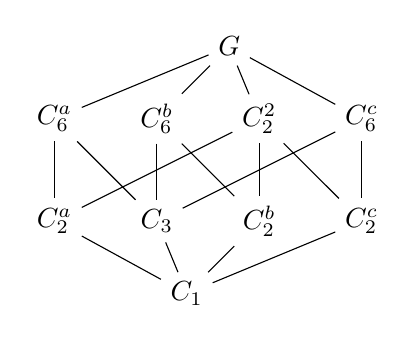
\begin{tikzpicture}[node distance=1.3cm]
        \node(G)[midway]{$G$};
        \node(C6b)[below left of =G]{$C_6^{b}$}; \node(C6a)[left of=C6b]{$C_6^{a}$};  
        \node(C22)[right of=C6b]{$C_2^{2}$};    \node(C6c)[right of=C22]{$C_6^{c}$};
        \node(C2a)[below of=C6a]{$C_2^{a}$};    \node(C3)[below of=C6b]{$C_3$};
        \node(C2b)[below of=C22]{$C_2^{b}$};    \node(C2c)[below of=C6c]{$C_2^{c}$};
        \node(C1)[below left of=C2b]{$C_1$};
        \draw(G)--(C6a);    \draw(G)--(C6b);    \draw(G)--(C6c);    \draw(G)--(C22);
        \draw(C6a)--(C2a);  \draw(C6a)--(C3);
        \draw(C6b)--(C2b);  \draw(C6b)--(C3);
        \draw(C6c)--(C2c);  \draw(C6c)--(C3);
        \draw(C22)--(C2a);  \draw(C22)--(C2b);  \draw(C22)--(C2c);
        \draw(C2a)--(C1);   \draw(C2b)--(C1);   \draw(C2c)--(C1);   \draw(C3)--(C1); 
    \end{tikzpicture}
    \end{figure}
    %There is a Brauer relation coming from the $C_2 \times C_2$-quotient, given by $$\Psi = C_3 - C_6^a - C_6^b - C_6^c + 2G.$$ 
    
    Consider an order $6$ character $\rho_a$ of $G$ with $C_2^{a}$ in its kernel. This has $\bQ(\rho_a) = \bQ(\zeta_6) = \bQ(\sqrt{-3})$. Let $\tau$ generate $\Gal(\bQ(\rho_a) / \bQ)$. One has
    \begin{equation}\label{ex1-rel}\tag{\textdagger}
    \Ind_{C_2^{a}}^G \trivial  \ominus \Ind_{C_6^{a}}^G \trivial \ominus \Ind_{C_2^{2}}^G \trivial \oplus \Ind_G^G \trivial \simeq \rho_a \oplus \rho_a^{\tau} .
    \end{equation}
    Let $E / \bQ$ be a semistable elliptic curve. To apply Theorem \ref{thm_positive_rank}, we need to compute
    \begin{equation}\label{ex1}\tag{*} 
        \frac{C_{E / F^{C_2^a}} C_{E / \bQ} }{C_{E / F^{C_6^a}} C_{E / F^{C_2^2}}} = 
        \frac{C_{E / L} C_{E / \bQ}}{C_{E / L^{C_3}} C_{E / L^{C_2}}}
    \end{equation} 
    where $L = F^{C_2^a}$ has $\Gal(L / \bQ) = C_6$, and check whether it is a norm from $\bQ(\sqrt{-3})$. This is a product of local Tamagawa numbers, as the minimal differential terms are $1$ when $E / \bQ$ is semistable (Lemma \ref{lem_Dterms}(i)). 
    
    One needs to compute these locally for each $p \in \bQ$. If $E / \bQ_p$ has good reduction, then the Tamagawa numbers at all places above $p$ in the subfields of $L$ are $1$. Suppose that $E / \bQ_p$ has split multiplicative reduction at $p$. Let $n = v_p(\Delta_E)$. For $H \leq G$, the Tamagawa number at a prime $\fP$ above $p$ in $L^H$ is given by $c_{\fp}(E / L^H) = e_{\fP \mid p} n$, where $e_{\fP \mid p}$ is the ramification degree. Thus the computation of Tamagawa numbers depends on the choice of decomposition group $D_p \leq C_6$ (to count the number of primes above $p$ in a given subfield) and the choice of inertia group $I_p \leq C_6$ (to compute the ramification indices). 
    
    The following table describes the product of Tamagawa numbers at places above $p$ in our expression, for varying $D_p$ and $I_p$. We let $T_{\fP \mid p}(E / L^H) = \prod_{\fP \mid p}c_{\fP}(E / L^H)$ for $H \leq \Gal(L / \bQ)$ as defined in Notation \ref{not_contr}. Let $C_p = c_p(E / \bQ)T_{\fP \mid p}(E / L) \big/ T_{\fP \mid p}(E / L^{C_3})T_{\fP \mid p}(E / L^{C_2})$. 
    \[
    \begin{array}{c c c c c c c}
        D_p & I_p & c_p(E / \bQ) & T_{\fP \mid p}(E / L^{C_3}) & T_{\fP \mid p}(E / L^{C_2}) & T_{\fP \mid p}(E / L) & C_p\\ 
        \hline
        C_1 & C_1 & n & n^2 & n^3 & n^6 & \square\\
        C_2 & C_1 & n & n & n^3 & n^3 & \square\\
        C_3 & C_1 & n & n^2 & n & n^2 & \square \\
        C_6 & C_1 & n & n & n & n & \square \\
        C_2 & C_2 & n & 2n & n^3 & (2n)^3 & \square \\
        C_6 & C_2 & n & 2n & n & 2n & \square \\
        C_3 & C_3 & n & n^2 & 3n & (3n)^2 & 3\cdot\square \\
        C_6 & C_3 & n & n & 3n & 3n & \square\\
        C_6 & C_6 & n & 2n & 3n & 6n & \square
    \end{array}
    \]

    In all cases we see that $C_p$, the contribution of Tamagawa numbers above $p$, is a norm form $\bQ(\sqrt{-3})$. It is not too hard to check that this is also the case when $E / \bQ_p$ has non-split multiplicative reduction. Therefore the expression in \eqref{ex1} is always a norm from $\bQ(\rho_a)$. This is an example of a more general phenomenon; for cyclic groups we always get a norm. This follows from  Theorem \ref{thm_consistent_cyclic}, which is proven in \S\ref{sec_cyclic}.
    %and $F / \bQ$ an abelian extension with $G = \Gal(F / \bQ)$. We claim that $C(\Theta) \in \fieldnorm{\rho_a}$, for all such $E$. Since each subgroup in $\Theta$ contains $C_2^{a}$, we have that $C(\Theta)$ equals $C(\Theta / C_2^{a})$ where $\Theta / C_2^{a} \in \B(G / C_2^{a}) = \B(C_6)$.  Now $\Theta / C_2^{a}$ is a $\chi_6$-relation, where $\chi_6 = \rho_a^{C_2^a}$ is a faithful order $6$ character of $C_6$, with $\bQ(\chi_6) = \bQ(\rho_a)$. But for cyclic groups we always get norm relations; by Theorem \ref{thm_consistent_cyclic}, $C(\Theta / C_2^{a}) \in \fieldnorm{\rho_a}$.

    But! Observe that{\footnote{this is called a Brauer relation, see Definition \ref{def-brauer}}} 
    \[ \Ind_{C_3}^G \trivial \ominus \Ind_{C_6^a}^G \trivial \ominus \Ind_{C_6^b}^G \trivial \ominus \Ind_{C_6^c}^G \trivial \oplus (\Ind_G^G \trivial)^{\oplus 2} = 0 \]
    as a virtual permutation representation. Append this to the left hand side of \eqref{ex1-rel}. Then Theorem \ref{thm_positive_rank} asks us to compute 
    \begin{equation}\label{ex1-rel2}\tag{**}
    \left(\frac{C_{E / F^{C_2^a}} C_{E / \bQ} }{C_{E / F^{C_6^a}} C_{E / F^{C_2^2}}}\right) \cdot \left( \frac{C_{E / F^{C_3}} C_{E / \bQ}^2}{C_{E / F^{C_6^a}}C_{E / F^{C_6^b}}  C_{E / F^{C_6^c}} } \right). 
    \end{equation}
    
    We can find instances where the second factor is not a norm from $\bQ(\sqrt{-3})$. Indeed suppose $E / \bQ$ has split multiplicative reduction at a prime $p$ with $D_p = G$, $I_p = C_6^b$. Let $v_p(\Delta_E) = n$. Then there is only one prime above $p$ in each subfield. Suppose $E$ has good reduction at all other primes (or multiplicative reduction at primes that are totally split in $F / \bQ$ would also be fine).
     Then our expression \eqref{ex1-rel2} is equal to
     \[ \frac{(6n)(n)}{(2n) (3n)} \cdot \frac{(2n)(n)^2}{(2n)(n)(2n)} \cdot \square = \frac{1}{2} \cdot \square, \] 
     which is not a norm from $\bQ(\sqrt{-3})$. Hence one must have $\rk E / F > 0$. 
\end{example}

\begin{example}[Dihedral]
    Let $q_1, q_2$ be odd primes. Consider $G = D_{2 q_1 q_2}$ the dihedral group of order $2 q_1 q_2$. 
    Let $\rho$, $\tau_1$, $\tau_2$ be two-dimensional irreducible representations of $G$ corresponding to rotating a $(q_1 q_2)$-gon by $2 \pi / q_1 q_2$, $2 \pi / q_1$, $2 \pi/ q_2$ respectively. These are all self-dual. The Galois conjugates of these representations, as well as the trivial $\trivial$ and sign $\epsilon$, yield all the irreducible representations of $G$. Let 
    \[  \sigma_{\rho} = \bigoplus_{ \fg \in \Gal(\bQ(\rho) / \bQ)} \rho^{\fg}, \qquad
        \sigma_1 = \bigoplus_{ \fg \in \Gal(\bQ(\tau_1) / \bQ)} \tau_1^{\fg}, \qquad
        \sigma_2 = \bigoplus_{ \fg \in \Gal(\bQ(\tau_2) / \bQ)} \tau_2^{\fg}. \]  
    Then $ \{ \trivial , \epsilon, \sigma_{\rho}, \sigma_1, \sigma_2 \}$ are a basis for the irreducible representations of $G$ over $\bQ$. 
    One has
\[
        \Ind_{C_2}^G \trivial \simeq \trivial \oplus \sigma_1 \oplus \sigma_2 \oplus \sigma_{\rho}, \quad
        \Ind_{D_{2 q_1}}^G \trivial \simeq \trivial \oplus \sigma_2, \quad
        \Ind_{D_{2 q_2}}^G \trivial \simeq \trivial \oplus \sigma_1,
\]
% There is an irreducible representation $\rho$ of $G$, obtained by inducing a linear order $q_1 q_2$ faithful representation from $C_{q_1 q_2}$. Thus $\rho$ is of degree $2$ and $\bQ(\rho) = \bQ(\zeta_{q_1 q_2})^{C_2}$. Then $\rho$ has $\frac{(q_1 - 1)(q_2 - 1)}{2}$ Galois conjugates, and so $\repnorm{\rho}$ is of dimension $2 \cdot \frac{(q_1 - 1)(q_2 - 1)}{2}$. 
and so 
\begin{equation*}
\Ind_{C_2}^G \trivial \ominus \Ind_{D_{2 q_1}}^G \trivial \ominus \Ind_{D_{2 q_2}}^G \trivial \oplus \Ind_{G}^G \trivial \simeq \bigoplus_{ \fg \in \Gal(\bQ(\rho) / \bQ)} \rho^{\fg}.
\end{equation*}

    Assume $E / \bQ$ is semistable. Suppose that $E / \bQ_p$ has split multiplicative reduction, with $n = v_p(\Delta_E)$. We compute Tamagawa numbers above $p$ as in the previous example, using the same notation. 
    Corollary \ref{cor-odd-decomp} implies that we always get a norm from the contribution above $p$ whenever the decomposition group is a group of odd-order. In fact we only get a non-square contribution when the decomposition group is $D_{2 q_1}$ or $D_{2 q_2}$ (and $I_p$ is non-trivial). 
     
    For example, let $p$ have decomposition group $D_{2 q_1}$ and inertia group $C_{q_1}$.
    This time, counting primes and computing ramification degrees is a little more awkward, we use Exercise \ref{ex-counting}.
        \begin{itemize}[--]
            \setlength\itemsep{0em}
            \item The action of $D_{2 q_1}$ on $C_2 \backslash G$ yields $1$ orbit of size $C_{q_1}$ (the orbit of the identity) and $\frac{q_2 - 1}{2}$ orbits of size $2q_1$ (coming from $C_2$ acting faithfully on $C_{q_2}$). The size of the inertia sub-orbits is $q_1$. Hence $T_{\fP \mid p}(E / F^{C_2}) = (q_1 n)^{1 + \frac{q_2 - 1}{2}}$.
            
            \item The action of $D_{2 q_1}$ on $D_{2 q_1} \backslash G$ yields the same number of orbits as above, but now the action of $C_{q_1} \leq D_{2 q_1}$ is trivial, so that $T_{\fP \mid p}(E / F^{D_{2 q_1}}) = n^{1 + \frac{q_2 - 1}{2}}$.
            
            \item The action of $D_{2 q_1}$ on $D_{2 q_2} \backslash G$ yields one orbit of size $q_1$, with the inertia sub-orbit also of size $q_1$, hence $T_{\fP \mid p}(E / F^{D_{2 q_2}}) = q_1 n$.
        \end{itemize}
    In total,
    \[ \frac{T_{\fP \mid p}(E / F^C_2) \cdot c_{\fp}(E / \bQ)}{T_{\fP \mid p}(E / F^{D_{2 q_1}})\cdot T_{\fP \mid p}(E / F^{D_{2 q_2}})} = \frac{(q_1 n )^{1 + \frac{q_2 - 1}{2}} (n)}{(n)^{1 + \frac{q_2 - 1}{2}} (q_1 n)} = q_1^{\frac{q_2 - 1}{2}} .\] 
    %By symmetry, taking the decomposition group to be $D_{2 q_2}$ and inertia group $C_{q_2}$, one would obtain $ q_2^{\frac{q_1 - 1}{2}}$.

    So let $E / \bQ$ have split multiplicative reduction at $p$ with decomposition group $D_{2 q_1}$ and inertia group $I_p = C_{q_1}$, and good reduction at all other primes. Further suppose that $q_1, q_2 \equiv 3 \pmod 4$ and that $\legendre{q_1}{q_2} = -1$. Then $\bQ(\sqrt{q_1 q_2}) \subset \bQ(\rho)$ but 
$$\frac{C_{E / F^C_2} C_{E / \bQ}}{C_{E / F^{D_{2 q_1}}} C_{E / F^{D_{2 q_2}}}} = q_1 \cdot \square$$
is not a norm from $\bQ(\sqrt{q_1 q_2})$. Indeed, $q_1$ is not the norm of an element of $\bQ(\sqrt{q_1 q_2})$, since $z^2 q_1 = x^2 - q_1q_2 y^2$ for $x,y,z \in \bZ$ implies $q_1 = \square \pmod {q_2}$, a contradiction. Thus $\rk E / F > 0$.

    This rank growth is predicted by root number computations also, however. Assume that $F / \bQ$ is totally real. Then $w(E / F^H) = (-1)^{[F^H \colon \bQ] + | H \backslash G / D_p|}$ by Proposition \ref{compute-root}. Thus
    \begin{itemize}[--]
        \setlength\itemsep{0em}
        \item $w(E / \bQ) = (-1)^2 = 1$,
        \item $w(E / F^{C_2}) = (-1)^{q_1 q_2} (-1)^{1 + \frac{q_2 - 1}{2}} = (-1)^{\frac{q_2 - 1}{2}}$,
        \item $w(E / F^{D_{2 q_1}}) = (-1)^{q_2}(-1)^{1 + \frac{q_2 - 1}{2}} = (-1)^{\frac{q_2 - 1}{2}},$
        \item $w(E / F^{D_{2 q_2}}) = (-1)^{q_1}(-1) = 1$. 
    \end{itemize}
    Therefore we must have $\rk E / F^{C_2}$, $\rk E / F^{D_{2q_1}} > 0$, so $\rk E / F > 0$. 
    Using the properties in Proposition \ref{compute-root-twist}, the computations of the root numbers for the subfields implies that 
    \[ w\left(E / \bQ, \sigma_1\right) = 1, \quad w\left(E / \bQ, \sigma_2\right) = -1, \quad w\left(E / \bQ, \sigma_{\rho}\right) = 1, \]
  and in particular $w(E / \bQ, \tau_1^{\fg}) = -1$ for some $\fg \in \Gal(\bQ(\tau_1) / \bQ)$.
\end{example}

\begin{example}[Additive reduction example]
Let $G = C_{65} \ltimes C_4$, where $C_4$ acts faithfully on $C_{65}$, as well as the subgroups $C_{13}$ and $C_5$. By inducing a faithful character of order $65$ from $C_{65}$, one obtains a faithful irreducible representation $\rho$ of $G$ of dimension $4$ and with $\bQ(\rho) = \bQ(\zeta_{65})^{C_4}$. In particular one has $\bQ(\sqrt{65}) \subset \bQ(\rho)$. Then
\[ \Ind_{C_4}^G \trivial \ominus \Ind_{C_{13} \ltimes C_4}^G \trivial \ominus \Ind_{C_5 \ltimes C_4}^G \trivial \oplus \Ind_{G}^G \trivial \simeq \bigoplus_{\fg \in \Gal(\bQ(\rho) / \bQ)} \rho^{\fg} .\]
Therefore by Theorem \ref{thm_positive_rank}, either 
\begin{equation}\label{ex3}\tag{\textdagger \textdagger}
\frac{C_{E / F^{C_4}} C_{E / \bQ} }{C_{E / F^{C_{13} \ltimes C_4}} C_{E / F^{C_5 \ltimes C_4}}}
\end{equation}
is a norm from $\bQ(\sqrt{65})$, or $\rk E / F > 0$.  

Suppose $p = 5$ and $E / \bQ_p$ has additive, potentially good reduction. Further suppose that $F / \bQ$ is an extension such that $D_{5} = I_{5} = C_5 \ltimes C_4$ (this is wildly ramified). Let $n = v_p(\Delta_E) < 12$. Then
\begin{itemize}[--]
    \setlength\itemsep{0em}
    \item In $F^{C_4}$ there is one prime above $p$ with ramification degree $5$ and $3$ primes above $p$ with ramification degree $20$,
    \item In $F^{C_{13} \ltimes C_4}$ there is one prime above $p$ with ramification degree degree $5$,
    \item In $F^{C_5 \ltimes C_4}$ there is one prime above $p$ with ramification degree $1$ and $3$ primes above $p$ with ramification degree $4$.
\end{itemize}
Therefore, by Lemma \ref{lem_Dterms}(iii), the product of the minimal differential term is 
\[ \frac{D_{\fP \mid p}(E / F^{C_4}) D_{\fP \mid p}(E / \bQ) }{D_{\fP \mid p}(E / F^{C_{13} \ltimes C_4}) D_{\fP \mid p}(E / F^{C_{5} \ltimes C_4})} = 
\frac{ 5^{\floor{5 n /12}} \cdot \left(5^{\floor{20 n /12}}\right)^3 }{5^{\floor{5 n /12}} \left(5^{\floor{4 n /12}}\right)^3} .\]
If $n = 2$, then this is equal to $5 \mod {(\bQ^{\times})^2}$. By Lemma \ref{tamagawa-num} the Tamagawa number product is
\[ \frac{T_{\fP \mid p}(E / F^{C_4}) T_{\fP \mid p}(E / \bQ) }{T_{\fP \mid p}(E / F^{C_{13} \ltimes C_4}) T_{\fP \mid p}(E / F^{C_{5} \ltimes C_4})} = \frac{1^2 \cdot 3^3 }{1^2 \cdot 3^3} = 1 \text{ or } \frac{1^5}{1^5} = 1.\]

We claim that $5$ is not a norm from $\bQ(\sqrt{65})$. Indeed, $5z^2 = x^2 - 65 y^2$ for $x, y, z \in \bZ$ implies that $5 = \square \pmod 13$, a contradiction since $\legendre{5}{13} = \legendre{13}{5} = \legendre{3}{5} = -1$. Therefore the local contribution of \eqref{ex3} above $5$ is not a norm from $\bQ(\sqrt{65})$. 

What are the local root numbers above $p$? By Proposition \ref{compute-root}, one has
\begin{itemize}[--]
    \setlength\itemsep{0em}
    \item $w(E / \bQ_5) = (-1)^{\floor{ 10 / 12}} = 1$, 
    \item $\prod_{\fp \mid p} w(E /F^{C_4}_{\fp}) = (-1)^{\floor{50 / 12}} \left((-1)^{\floor{200 / 12}}\right)^3 = 1$,
    \item $\prod_{\fp \mid p} w(E /F^{C_{13} \times C_4}_{\fp}) = (-1)^{\floor{50 / 12}} = 1$,
    \item $\prod_{\fp \mid p}w(E /F^{C_{5} \times C_4}_{\fp}) = (-1)^{\floor{ 10/12}}\left((-1)^{\floor{40 / 12}}\right)^3 = -1$ .
\end{itemize}
Hence we see a change in the contributions of local root numbers above $p$ in the intermediate subfields. 




\end{example}


\section{Consistency cases with BSD}
As we discussed in the previous section, our motivation is to use Theorem \ref*{thm_positive_rank} to predict points of infinite order for families of elliptic curves. However, in this section we prove that in several cases the theorem will never make such a prediction. In other words, in such cases, the product 
$$\frac{\prod_i C_{E/F_i}}{\prod_j C_{E/F_j'}}$$ 
is always a norm for every subfield $\QQ(\sqrt{D})\subseteq\QQ(\rho)$.

\subsection{Cyclic Extensions}
In this subsection we prove the following. 
\begin{thm}\label{thm_consistent_cyclic}
    Let $E/\QQ$ be a semistable elliptic curve and let $F$ a finite cyclic Galois extension over $\QQ$ so that $\Gal(F/\QQ)=C_d$ for some $d\geq 2$. Let $\chi$ be a faithful character of $C_d$ (so that $\QQ(\chi)=\QQ(\zeta_d)$), and let $F_i,F'_j\subseteq F$ be such that
    $$\bigoplus_{\mathfrak{g}\in\Gal(\QQ(\zeta_d)/\QQ)}\chi^{\mathfrak{g}}=\bigoplus_i\Ind_{F_i/\QQ}\mathds{1}\ominus\bigoplus_j\Ind_{F'_j/\QQ}\mathds{1}.$$
    Then for any $\QQ(\sqrt{D})\subseteq\QQ(\zeta_d)$,
    $$\frac{\prod_i C_{E/F_i}}{\prod_j C_{E/F_j'}}$$
    is a norm of $\QQ(\sqrt{D})$.
\end{thm}

The first step in proving Theorem \ref*{thm_consistent_cyclic} is to show that the fields $F_i, F'_j$ exist, and to give a precise description. Recall that for each $k\mid d$ the cyclic group $C_d$ has one unique subgroup of order $k$, which is of course also cyclic. Therefore, for each $k\mid d$, there is one unique subfield $F_k$ of $F$ of degree $k$ over $\QQ$ which is also cyclic. The corresponding subgroup $H_k=\Gal(F/F_k)=C_{d/k}$.

To give the required description, we recall that the Möbius function $\mu$ is the function supported on the square-free integers, and $\mu(n)=(-1)^s$ whenever $n$ is square free and $s$ is the number of prime factors of $n$.

\begin{lemma}
    Let $E/\QQ$, $F$ and $\chi$ be as in Theorem \ref*{thm_consistent_cyclic}. Writing characters of $C_d$ additively, we have that
    \begin{equation}
        \sum_{\mathfrak{g}\in\Gal(\QQ(\zeta_d)/\QQ)}\chi^{\mathfrak{g}}=\sum_{k\mid d}\mu(d/k)\Ind_{F_k/\QQ}\mathds{1}.
    \end{equation}
\end{lemma}

\begin{proof}
    The proof is essentially application of Frobenius reciprocity and the inclusion exclusion lemma. Let $p_1,\ldots,p_s$ be the distinct primes dividing $d$. By Frobenius reciprocity, for any character $\theta$ of $C_d$ and $k\mid d$,
    $$\langle\theta,\Ind_{F_k/\QQ}\mathds{1}\rangle_{C_d}=\langle\Res_{F_k/\QQ}\theta,\mathds{1}\rangle_{C_{d/k}}.$$
    That is, $\theta$ appears as a factor of $\Ind_{F_k/\QQ}\mathds{1}$ if and only if $\chi|_{C_{d/k}}$ is trivial, and it can only appear once. Therefore,
    $$\Ind_{F_k/\QQ}\mathds{1}=\sum_{\theta\in\mathcal{A}_{d/k}}\theta$$
    where $\mathcal{A}_k=\{\theta\in\widehat{C_d}:\theta|_{C_{k}}=\mathds{1}_{C_{k}}\}$. Note that if $k,k'\mid d$ are coprime, then $\mathcal{A}_k\cap\mathcal{A}_{k'}=\mathcal{A}_{kk'}$. If $\mathcal{B}$ is the set of faithful characters of $C_d$, then by the inclusion-exclusion lemma
    %\begin{multline*}
    %    \sum_{\theta\in\mathcal{B}}\theta=&\sum_{i=0}^s(-1)^i\sum_{1\leq j_1\leq\dots\leq j_i\leq s}\ \sum_{\theta\in\cap_{l=1}^i\mathcal{A}_{p_{j_l}}}\theta\\
    %    =&\sum_{i=0}^s(-1)^i\sum_{1\leq j_1\leq\dots\leq j_i\leq s}\ \sum_{\theta\in\mathcal{A}_{\prod_{l=1}^i p_{j_l}}}\theta\\
    %    =&\sum_{k\mid d}\mu(k)\sum_{\theta\in\mathcal{A}_k}\theta=\sum_{k\mid d}\mu(d/k)\Ind_{F_k/\QQ}\mathds{1}.
    %\end{multline*}
    The proof now follows from the fact that if $\chi$ is a faithful character, then the set $\{\chi^{\mathfrak{g}}:\mathfrak{g}\in\Gal(\QQ(\zeta_d)/\QQ)\}$ spans over all faithful characters of $C_d$ once. 
\end{proof}


\subsection{Abelian Extensions}

\subsection{Odd-Degree Extensions}



\newpage

\bibliography{references.bib}
\bibliographystyle{amsalpha}


\end{document}